% !TEX root = ../../book.tex
\chapter{Statistical Trading Strategies and Back-Testing\label{ch:stat_ts}}
\section{Introduction to Trading Strategies: Origin and History}

\noindent\textbf{Statistical arbitrage opportunity and strategies:} Trading strategies are central to the notion of statistical arbitrage. Strategies that claim to have better performance than the market date back to the inception of trading in finance. This area under the name of `technical analysis' is based on using past prices and other stock and market-related statistics to make investment decisions. The ideas date back to a Japanese speculator, Munehira Homma, who made a fortune in the rice market using techniques called candlestick patterns. The famous Dow Theory is based on the assertion that the market in certain phases can be predictable. Thus, there is a history of studies that empirically conclude that the behavior of stock prices appear to contradict efficient market hypothesis. Broadly, there are two types of strategies, one the momentum strategy that  advocates buying well-performing stocks and selling poor-performing stocks (see Jegadeesh and Titman (1993)~\cite{JeTit}) and the other, contrarian or reversal strategy that advocates buying past losers and selling past winners. The average excess return of some strategies relative to an `alpha' in a standard capital asset pricing model is shown to be around 12\%. Other strategies, known as value strategies suggest buying value and selling glamour stocks (see Lakonishok et al. (1994)~\cite{Lako}). They use other company fundamental data such as price earnings ratios, dividends, book-to-market values, cash flows and sales growth. A measure of value is the ratio of book value or earnings to market price.


Hogan, Jarrow, Teo and Warachka (2004)~\cite{Hogan} define `a statistical arbitrage as a long horizon trading opportunity that generates a riskless profit. Four conditions that are to be met are: it is a self-financing strategy with a zero initial cost, in the limit has positive expected discounted profits, a probability of a loss converging to zero and a time-averaged variance converging to zero; the last condition implies that an arbitrage opportunity eventually produces riskless profit. Citing anomalies to reject  market efficiency has been criticized on the ground that such tests depend upon a specified model for equilibrium returns. Hogan et al. (2004)~\cite{Hogan} argue that statistical arbitrage can be defined without any reference to an equilibrium model and rejects market efficiency. They provide a statistical test to determine if a trading strategy constitutes statistical arbitrage based on short horizon incremental profits. Some issues that arise in developing and testing strategies are: handling the transaction costs both direct, such as brokerage fee, and indirect due to the entry/exit to the market; cross-validation to avoid over-fitting; no guaranteed performance in different market settings. In this chapter, we will cover some of these trading strategies and finally we will return to the proposed statistical test.



% Trading Rules for Time Aggregated Data
\section{Trading Rules for Time Aggregated Data \label{s:trading_rules_tad}}


Trading Rules that are broadly labeled under technical analysis involve the prediction of future short-term price movements from an inductive analysis of past movements using either quantitative techniques, such as moving averages or qualitative methods such as pattern recognition from visual inspection of a time-series plot of the asset price data or a combination of both via semi-parametric procedures such as kernel smoothing. In foreign exchange market, as Menkhoff and Taylor (2002)~\cite{MalTay} observe the widespread use of these techniques is puzzling, ``since technical analysis eschews scrutiny of economic fundamentals and relies on information on past exchange rate movements that, according to the weakest notion of market efficiency, should already be embedded in the current exchange rate, making its use either unprofitable or implying that any positive returns that are generated are accompanied by an unacceptable risk exposure.'' In general there are economic fundamentals that can explain long term movements, there is still no fundamental-based exchange rate model that is capable of forecasting short-term movements.


Technical analysis (also known as Chartist analysis) is a set of techniques for obtaining forecasts based on past history of prices along with the history of trading volumes. Clearly for the technical analysis to be useful, price movements should follow some regular, recurring patterns and these patterns must hold for long enough periods to sustain the transaction costs and false signals so that the investment results in a profit. What constitutes a useful forecast from an investor point of view could be if the past history of prices can be used to increase expected gains. But as Fama and Blume (1966)~\cite{famablume} point out, ``In a random walk market, with either zero or positive drift, no mechanical trading rule applied to an individual security would consistently outperform a policy of simply buying and holding the security''. The past movements could be useful only when there is some degree of dependence in successive price changes. The serial correlation measures may not capture the complex dependence that may exist. In what follows we briefly describe some commonly used trading rules and comment on their noted performance.



% Filter Rules
\subsection{Filter Rules}


Alexander (1961, 1964)~\cite{alexander61,alexander64} studied the filter technique that is intuitive and is easy to implement; the basic idea is summarized below: \twomedskip


\fbox{%
\begin{minipage}{0.90\textwidth}
\noindent\textbf{x\% Filter:} If a daily closing price moves up at least x\% from its past low, buy and hold, until its price moves down at least x\% from a subsequent high, sell and go short. Maintain the short position until price rises at least x\% above a subsequent low, buy. Moves less than x\% in either direction are ignored.
\end{minipage}
} \twomedskip


The general logic behind this rule is that if the price moved up $x$\%, it is likely to move up more than $x$\% further before it moves down by $x$\%; Thus the random walk model is not likely to be upheld by the data. As observed by Mandelbrot (1963)~\cite{mandelbrot}, because of the price jumps that occur at the time of transaction, the purchase price and sale price will not exactly match as required by the rule.


The initial application of this rule on daily data for S\&P industrials showed that the trading rules with 5, 6 and 8\%. filters generated larger gross profits than the buy and hold strategy. This study did not account for the transaction cost. But a later study that incorporated a commission of 2\% for each round-trip, only the larger filter  $\sim$ 46\% rule beat the buy and hold strategy and all the other filters adjusting for the transaction costs did not perform better than simply buying and holding.


Fama and Blume (1966)~\cite{famablume} after applying Alexander's filter technique for each of the individual security in Dow Jones Industrial Average for the daily data during a five year period, 1957--1962, concluded, ``When commissions are taken into account, the larger profits under the filter technique are those of the brokers. When commissions are omitted, the returns from the filter techniques are, of course, greatly improved but are still not as large as the returns from simply buying and holding.'' It is argued that under random walk model, the average return on long positions should be approximately equal to the buy and hold average returns. This may not be true if the drift occurs at the time of entry or exit; the filter rule can be stated under RW Model as follows; let the return, $r_{t} = \ln{P_{t}} - \ln{P_{t-1}} = \mu_{t} + a_{t}$, when $a_{t} \sim$ N(0,$\sigma_{a}^2$) and `$\mu_{t}$' is the random drift term and $\sigma_{a}^2$ is the volatility; as for the filter rule, enter if $r_{t} > r$ and suppose this occurs at time $t_{0}$. If the drift term is approximately picked up at time `$t_{0}$', so that $\mu_{t} = 0$, for $t < t_{0}$ but $\mu_{t} = \mu > 0$ for $t \geq t_{0}$, the returns from the filter should fare better. The lasting of the drift is to be carefully monitored and using the exit strategy when $r_{t} < r$ will guarantee any undue losses.


When the filters are small it has been observed that there is evidence of positive dependence in returns and it may be useful to predict only short term dependence. This may signal opportunities for more frequent transactions but the cost of transactions as mentioned earlier can eat away the profits.


Sweeney (1988)~\cite{sweet} develops a test for risk-adjusted filters profits. The stocks considered in Fama and Blume (1966)~\cite{famablume} that are ``winners'' in one period tend to persist as winners in later periods as well. Thus focusing only on winners rather than entire set of stocks gives better results. Assume that the investor uses the filters rule each day to decide to enter or exit based solely as past information. Consider the span of $N$ days and with a filter strategy, the asset is held on $N_{\text{in}}$ days and is not held on $N_{\text{out}}$ days. At the end of $N$ days, the filter's performance is evaluated. The average excess rate of buy and hold is
	\[
	\overline{R}_{\text{BH}}=\dfrac{1}{N} \sum_{i=1}^N \, (r_t - r_f ),
	\]
where $r_t$ is the stock's rate of return in period `$t$' and $r_f$ is the risk free rate. Assume that `$f$' is the proportion of days, the asset is not held; then the average excess rate of the filter is
	\[
	\overline{R}_{F}=\dfrac{1-f}{N_{\text{in}}} \sum_{t \in I} (r_t - r_f).
	\]
Assume that under any of the asset pricing models (CAPM, APT etc.) expected excess rate of return equals a constant risk premium, $\text{PR}_{j}$. Note $E(\overline{R}_{\text{BH}}) = \text{PR}$ and $E(\overline{R}_{F}) = (1 - f)\,\text{PR}$; Use the adjusted statistic
	\begin{equation} \label{eqn:xbarfirst}
	x= \overline{R}_{F} - (1 - f)\, \overline{R}_{\text{BH}}
	\end{equation}
to judge the filter rule; observe $E(x) = 0$ and $\sigma_{x} = \sigma[\frac{f(1-f)}{N}]^{1/2}$, where `$\sigma$' is the standard deviation of excess return $r_t - r_f$. Fama and Blume (1966)~\cite{famablume} use
	\begin{equation} \label{eqn:bigxbar}
	X = \overline{R}_{FI} - \overline{R}_{BH}
	\end{equation}
where $\overline{R}_{fI} = \frac{1}{N_{\text{in}}} \sum_{t \in I}(r_t - r_F)$; Note $E(X) = 0$ and $\sigma_{x} = \sigma_{X}$.


The main advantage of $X$ is that it measures profits for each day in the duration of `$N$' days and $x$ measures profits per day for those days when the stock is held. The above results hold for the case of time varying risk premia as well; Suppose
	\[
	R_f - r_f = \text{PR} + a_t,
	\]
where $a_t$ is stochastic; thus
	\begin{equation} \label{eqn:anotherxeq}
	x = \dfrac{1}{N_{in}} \sum_{t \in I} a_t - \dfrac{1}{N} \sum_{t=1}^N a_t + (\overline{\text{PR}}_{N_{in} }+\overline{\text{PR}}_N ).
	\end{equation}
If the investor has no insight into changes in risk premia, then $E(\overline{\text{PR}}_{N_{\text{in}}} - \overline{\text{PR}}_{N}) = 0$; If the investor has no insight about the stochastic, $a_t$, the filter rule may be forecasting the risk premia.


It has been pointed out that Fama and Blume measure is biased against finding successful filter rules. The statistics $X$ and $x$ are meant for long strategies where the investor has the funds in the risk free asset when not holding. If we define,
	\[
	\overline{R}_{F'} = \dfrac{1}{N} \left( \sum_{t\in I} (r_t - r_f) - \sum_{t \in O} (r_t - r_f) \right)
	\]
and $E(\overline{R}_{{F}'} - \overline{R}_{\text{BH}}) = (1 - 2f) \text{PR} - \text{PR} = -2f \text{PR}$, a proportion of constant risk premium, thus resulting in a bias.



% Moving Average Variants and Oscillators
\subsection{Moving Average Variants and Oscillators}


The moving average trading rules are generally based on comparing the current price with a form of current moving average. Consider the prices, $P_t, P_{t-1}, \ldots, P_{t-m+1}$ with a moving window of width `$m$'. Various versions of moving average are available in the literature and their relative merits depend on the pattern of time series data:
	\begin{flalign}\label{eqn:multi}
	&& &\text{(SMA)} && \notag \\
	&& &\text{Simple Moving Average: } \overline{P}_t^{(m)}= \dfrac{1}{m} \sum_{i=0}^{m-1} P_{t-i} && \notag \\
	&& &\text{(EWA)} && \notag \\
	&& &\text{Exponentially Weighted Average: } \overline{P}_t^{(m)} = \left(\dfrac{1}{\sum_{i=0}^{m-1} \lambda^{i+1}} \right) \sum_{i=0}^{m-1} \lambda^{i+1} P_{t-i} && \\
	&& &\text{(BWA)} &&  \notag \\
	&& &\text{Bollinger Weighted Moving Average: }  \hat{P}_t^{(m)}= \left(\dfrac{1}{\sum_{i=1}^m i}\right) \sum_{i=0}^{m-1} (m-i) P_{t-i} && \notag
	\end{flalign}
Note that $0 < \lambda < 1$. The indicators of the above kind will tend to be profitable in markets that exhibit definite trends and so they are generally known as ``trend-following'' or some times, called as ``momentum'' indicators. Some simple rules that are normally used in practice are: \twomedskip


\noindent\fbox{%
    \parbox{\textwidth}{%
	\textbf{SMA Rule: If } $\mathbf{\frac{\overline{P}_{t}^{(m)}}{P_{t}} > U} \textbf{ or }\mathbf{<L,}$ \textbf{ trade;} \twomedskip
	
	\textbf{EWA Rule: If } $\mathbf{\frac{\overline{P}_{t}^{(m)}(\lambda)}{P_{t}} > U} \textbf{ or }\mathbf{<L,}$ \textbf{ trade}
    }%
} \twomedskip


The two types of potential strategies are broadly known as ``Reversed'' vs ``Momentum'' and they differ mainly on when the entry is carried out. The contrarian in a way looks for local minimum to enter the market and the momentum follower looks for a local maximum to enter.


While the above rules are easy to implement and one may observe that they do not take into account the variance or the volatility of the price (return) process. The widely used Bollinger band, conceptually similar to monitoring the quality of a manufacturing process, is based on the weighted moving average and the variance. Define the standard deviation as, $\hat{\sigma}_{t}^{(m)} = \{ \frac{1}{m-1} \sum_{i=0}^{m-1} (P_{t-i} - \overline{P}_{t}^{(m)})^2 \}^{1/2}$ and the rule can be stated as follows: \twomedskip


\noindent\fbox{%
    \parbox{\textwidth}{%
	\textbf{Bollinger Rule: If }$\mathbf{P_{t} > P_{t}^+ = \hat{P}_{t}^{(m)} + 2\hat{\sigma}_{t}^{(m)}}$\textbf{, the upper band, then sell; if } $\mathbf{P_{t} < P^- = \hat{P}_{t}^{(m)} - 2\hat{\sigma}_{t}^{(m)}}$ \textbf{, the lower band, then buy; No action is taken in-between.}
    }%
} \twomedskip


Broadly the key quantities such as moving average, weighted (exponentially or otherwise) average, etc. correspond to the running-mean smoother discussed in Lai and Xing (2009)~\cite[Section 7.2.1]{lai1}. Instead of the running-mean, some technical rules use the running maximum (i.e. $\max\limits_{0 \leq i \leq m} P_{t-i}$) or the running minimum (i.e., $\min\limits_{0 \leq i \leq m} P_{t-i}$) in the above rules. \twomedskip


\noindent\textbf{Moving Average Oscillator:} The use of the technical rules by the foreign exchange professionals is well documented (See Menkhoff and Taylor (2007)~\cite{MalTay}). The so-called moving average oscillator rule requires computing two moving averages of short and long time spans. Let $\overline{P}_{t}^{(m)}$ and $\overline{P}_{t}^{(n)}$ be the short and long averages, where $m< n$. The rule would signal a break in trend when the longer moving average is crossed by a shorter moving average (or spot rate). The upward trend is signaled when short moving average intersects from below the long average. Conversely, a downward break in trend is signaled if the crossing occurs from above. Precisely the rule is: \twomedskip


\noindent\fbox{%
    \parbox{\textwidth}{%
\noindent\textbf{Oscillator Rule: } \twomedskip

\noindent\textbf{Enter if } $\mathbf{\overline{P}_{t-1}^{(m)} < \overline{P}_{t-1}^{(n)}}$ \textbf{ and } $\mathbf{\overline{P}_t^{(m)} > \overline{P}_t^{(n)}}$ \twomedskip

\noindent\textbf{Exit if }$\mathbf{\overline{P}_{t-1}^{(m)} > \overline{P}_{t-1}^{(n)}}$ \textbf{ and }$\mathbf{\overline{P}_t^{(m)} < \overline{P}_t^{(n)}}$ \twomedskip
    }%
} \twomedskip


\noindent\textbf{RSI Oscillator:} Another oscillator that is designed to measure the strength of price movement in a particular direction is the relative strength indicator (RSI). The logic being that if the changes in price are too rapid in one direction, a correction in the opposite direction is likely to follow and occur soon. Thus these types of rules are called `reversal' or `overbought/oversold' indicators. To define RSI, let $U_{t} = \sum_{i=1}^m I(P_{t-i} - P_{t-i-1} > 0)\,\lvert P_{t-i} - P_{t-i-1} \rvert$ and $D_{t} = \sum_{i=1}^m I_{t} (P_{t-i} - P_{t-i-1} < 0)\,\lvert S_{t-i} - S_{t-i-1}\rvert$ where $I(\cdot)$ is an indicator function. Thus $U_t$ and $D_t$ aggregate the positive and negative side of the price changes. Now let $\text{RS}_{t} = \frac {U_{t}}{D_{t}}$, and can be taken as a measure of odds ratio, and define
	\begin{equation} \label{eqn:rsi}
	\text{RSI}_{t} = 100 \times \frac{U_{t}}{U_{t} + D_{t}} = 100 - 100 \left( \dfrac{1}{1 + \text{RS}_t} \right).
	\end{equation}
By construction, RSI is normalized and it takes values between 0 and 100. \twomedskip


\noindent\fbox{%
    \parbox{\textwidth}{%
\noindent \textbf{Reversal Rule:} \twomedskip

\noindent\textbf{If }$\mathbf{RSI_{t} > 70}$\textbf{, it is overbought signaling a downward correction and hence exit or short sell.} \twomedskip

\noindent\textbf{If }$\mathbf{RSI_{t} < 30}$\textbf{, it is oversold signaling an upward correction and hence enter.} \twomedskip
    }%
} \twomedskip


These rules that appear to be somewhat ad hoc can all be related back to the random walk model (see Chapter~\ref{ch:ch_uvts}) possibly with a drift:
	\begin{equation} \label{eqn:anotherpt}
	p_t = \mu + p_{t-1} + a_t,
	\end{equation}
where $a_t \sim \text{N}(0,\sigma^2)$, $\sigma^2$ is the volatility of the stock and note the return, $r_t= p_t - p_{t-1}$; thus, $r_t \sim \text{N}(\mu,\sigma^2)$. If there is any autocorrelation in `$r_t$', and if $\overline{r}_n$ is the average based on the last `$n$' observations, then $\overline{r}_n \sim \text{N}\left(\mu,\sum_{\mid h \mid < n}\left(1-\frac{\mid h \mid}{n}\right)\frac{\gamma(h)}{n}\right)$, where $\gamma(h)$ is the autocovariance function of lag `$h$', with $\gamma(0)=\sigma^2$. When $\gamma(h)=0 \text{ for } h > 0$, that P($\overline{r}_n > 0)= \text{P}(\overline{a}_n > -\mu)= \text{P}\left( \frac{\overline{a}_n}{\sigma} > \frac{-\mu}{\sigma} \right)= 1 - \Phi\left( -\frac{\mu}{\sigma} \right)$, where $\Phi$ is the c.d.f. of the standard normal distribution. Thus we can evaluate $RS_t$ by the odds ratio, $(1 - \Phi(-\frac{\mu}{\sigma}))/(\Phi(-\frac{\mu}{\sigma}))$. In fact the reversal rule stated above implies for $RSI_t$ to be greater than 70, $\text{RS}_t > 2.33$. All the rules stated in this section can be written in the form of the c.d.f. of the underlying distribution of the return. This model-based interpretation of the rules can help us in accommodating other factors such as volume more formally in the model and their value added in the strategy performance. 



% Patterns Discovery via Non-Parametric Smoothing Methods
\section{Patterns Discovery via Non-Parametric Smoothing Methods}


Charting has been a part of financial practice for many decades; but because of its highly subjective nature of interpretation of geometric shapes in price series, reading charts is ``often in the eyes of the beholder''. Lo, Mamaysky and Wang (LMW) (2000)~\cite{LoMWang} propose a systematic approach to pattern recognition using nonparametric kernel regression. The general goal of this analysis is to identify regularities in the price series by extracting nonlinear patterns. The smoothing estimators that can extract the signal by averaging out the noise are ideally suited for this task.	


Assume that prices follow,
	\begin{equation} \label{eqn:4pt}
	P_{t} = m(x_{t}) + a_{t},
	\end{equation}
where $m(x_{t})$ is an arbitrary function of the state variable, $X_{t}$. For most practical purposes, assume $X_{t}= t$ as the data is typically chronological. Kernel regression, orthogonal series expansion, projection pursuit, neural networks are all examples of smoothing methods that are applied to estimate $\hat{m}(x_{t})$;
	\begin{equation} \label{eqn:4mx}
	\hat{m}(x) = \frac{1}{T} \sum_{t=1}^Tw_{t}(x)P_{t},
	\end{equation}
where the weights $\{w_{t}(x)\}$ are large for those $P_{t}$'s paired with $x_{t}$'s near $x$ and are small for those away from $x$. The weight function in \eqref{eqn:4mx} is defined for a neighborhood of width `$h$'  around `$x$' can be stated as
	\begin{equation} \label{eqn:3mhat}
	\hat{m}_{h}(x) = \frac{1}{T}\sum_{t=1}^T w_{t,h}(x)P_{t} = \dfrac{\sum_{t=1}^T K_{h}(x-x_{t})P_{t}}{\sum_{t=1}^T K_{h}(x-x_{t})},
	\end{equation}
where $K(x)$ is a probability density function and is also-called as `Kernel', and $\hat{m}_{h}(x)$ is called Nadaraya-Watson kernel estimator. A popular density is that of a standard normal distribution, $K(t)=\frac{e^{-t^2/2}}{\sqrt{2\pi}}$.


Selecting the appropriate bandwidth, `$h$' is important as a small `$h$' may not smooth much and a large `$h$' may result in too smooth a graph. The choice of `$h$' is made through cross-validation, by minimizing
	\begin{equation} \label{eqn:cvh}
	\text{CV}(h) = \frac{1}{T}\sum_{t=1}^T (P_{t} - \hat{m}_{h}(t))^2,
	\end{equation}
where
	\begin{equation} \label{eqn:mht}
	\hat{m}_{h,t} = \frac{1}{T}\sum_{\tau\not=t}^T w_{\tau,h}P_{\tau}.
	\end{equation}
Thus, the bandwidth choice depends on empirically how well the estimator fits each observation, $P_{t}$, when it is not used in the construction of a Kernel estimator. LMW(2000)~\cite{LoMWang} observe that generally the bandwidth choice made through \eqref{eqn:cvh} when applied to price series, tend to be larger and they suggest using $0.3 \times h$.


To automate the detection of charting patterns, first the pattern is defined in terms of its geometric properties, then $\hat{m}(x)$ is estimated via \eqref{eqn:3mhat}, to match with it. LMW(2000)~\cite{LoMWang} define ten different patterns based on local extremes. The window size is $(t,t+l+d-1)$, where $l$ and $d$ are fixed parameters, so that a pattern is completed within $l+d$ trading days. Within each window, estimate  a kernel regression using prices in that window:
	\begin{equation} \label{eqn:longhat}
	\hat{m}_{h}(\tau) = \dfrac{\sum_{s = t}^{t+l+d-1}K_{h}(\tau - s)P_{s}}{\sum_{s = t}^{t+l+d-1}K_{h}(\tau - s)}, \quad t = 1,\ldots , T-l-d-1
	\end{equation}
and the local extremes are identified through sign changes in $\hat{m}_{h}(\tau)$.


To test if the kernel regression yields better prediction, LMW(2000)~\cite{LoMWang} compare the unconditioned distribution of returns to the conditioned distribution, conditioned on the existence of a pattern. These comparisons are made through a goodness-of-fit test such as Kolmogorov-Smirnov test. It  is generally found that the Kernel regression method yields somewhat better predictions. Jegadeesh (2000)~\cite{Jeqa} in his discussion of LMW(2000)~\cite{LoMWang} questions if the chartists' belief that selected patterns of the past tend to repeat as there is a great deal of noted subjectivity in the interpretation of charts. It is further noted that the practitioners tend to use the visual patterns in conjunction with other information such as macro level events that exert large influence compared to stock specific moves, to time their trades.



% A Decomposition Algorithm
\section{A Decomposition Algorithm \label{s:decomp_alg}}


The rules that were discussed in previous sections are mostly trend following and use the past price or returns data. The predictability of returns generally tends to be weak consistent with efficient market theory. But the direction of change and volatility of returns tend to exhibit somewhat stronger dependence over time. Anatolyev and Gospodinov (2010)~\cite{Ananto2} exploit this and decompose the returns into a product of sign and absolute value components whose joint distribution is obtained through a model for absolute value of the return and a binary choice model for direction of the return and a copula for their interaction. Precisely the returns, `$r_{t}$', is written as
	\begin{equation} \label{eqn:3sgn}
	r_t = c + \lvert r_t - c\rvert \sgn (r_t - c)= c + \lvert r_t - c \rvert (2\cdot I(r_t  > c) - 1),
	\end{equation}
where $I(r_t > c)$ is an indicator function. The values of $c$ are determined by the user; it could be a multiple of the standard deviation of `$r_{t}$' or it could represent the transaction cost or the risk free rate. This model is conceptually similar to Rydberg and Shephard (2003)~\cite{Ryd} and potential usefulness of the decomposition is also mentioned in Anatolyev and Gerko (2005)~\cite{Ananto1}.


An advantage of the decomposition can be illustrated as follows. Assume for convenience, $c = 0$. From the model for $|r_t|$ and $I(r_t > 0)$, write $E_{t-1}(\left|r_{t}\right|) = \alpha_{\left|r\right|} + \beta_{\left| r \right|}\text{RV}_{t-1}$ and $\text{Pr}_{t-1}(r_t >0) = \alpha_{\left| I \right|} + \beta_{\left| I \right|}\text{RV}_{t-1}$, where RV denotes the realized volatility resulting in 
	\[
	E_{t-1}(r_t)= -E_{t-1}(\left| r_t \right|) + 2E_{t-1}(\left| r_{t} \right| \cdot I(r_{t} > 0))= \alpha_{r} + \beta_{r} \text{RV}_{t-1} + \sigma_{r} \text{RV}_{t-1}^2.
	\]


Thus, the decomposition in \eqref{eqn:3sgn} leads to accommodating non-linearity and the model can be expanded to include other asset related variables. Hence any dynamic modeling that captures the hidden non-linearities is likely to improve the prediction of $r_{t}$. With the random walk model for price, $r_t$ is taken to be white noise, but the above formulation helps to capture any time dependence. We describe below some useful formulations.


The marginal distributions of the absolute value and sign terms are modeled as follows.
	\begin{equation} \label{eqn:psieta}
	\lvert r_{t} - c \rvert = \psi_{t} \eta_{t},
	\end{equation}
where $\eta_{t}$ is Weibull distribution and
	\begin{equation} \label{eqn:lnspi}
	\ln{\psi_{t}} = w_{v} + \beta_{v} \ln{\psi_{t-1}} + r_{v} \ln\lvert r_{t-1} - c \rvert + \rho_{v} I(r_{t-1}>c) + x'_{t-1} \delta_{v}.
	\end{equation}
Note the above specification is the same as the autoregressive conditional duration (ACD) model discussed in Chapter~\ref{ch:ch_advanced}. The $x_{t}$'s  are macroeconomic predictors that may have an effect on volatility dynamics. The specification of the indicator variable is done as follows: The indicator variable $I(r_{t} > c)$ is assumed to follow Bernoulli($p_{t})$, where $p_{t} = \text{logit}(\theta_{t})$, where 
	\begin{equation}\label{eqn:3thetat}
	\theta_{t} = w_{d} + \phi_{d}I (r_{t-1}>c) + y_{t-1}'\delta_{d},
	\end{equation}
where the $y_{t}$'s can, besides the macro economic variables, include the realized variance, $\text{RV}_{t} = \sum_{s=1}^{m} r^2_{t,s}$, bipower variation, $\text{BPV}_{t} = \frac{\pi}{2} \cdot \frac{m}{m-1} \cdot \sum_{s=1}^{m-1} \lvert r_{t,s}\rvert\, \lvert r_{t,s+1}\rvert$ and the realized third and fourth moments representing skewness and kurtosis measures, $\text{RS}_{t} = \sum_{s=1}^m r_{t,s}^3$ and $\text{RK}_{t} = \sum_{s=1}^{m} r_{t,s}^4$.


With the marginals specified as above with the corresponding, c.d.f.'s $F(\cdot$), the joint density is given as
	\begin{equation}\label{eqn:frt}
	F_{r_t}(u,v) = c \left[ F_{\lvert r_t-c\rvert}^{(u)}, F_{I(r_t>0)}^{(v)} \right]
	\end{equation}
where $c(w_1, w_2)$ is a Copula, a bivariate c.d.f.. For a general discussion on Copulas, refer to Lai and Xing (2008)~\cite[Section 12.3.3]{lai1}.


In the trading context, the value of a strategy to buy or sell depends on how good the short term prediction of $r_{t}$ is. Note that the conditional mean can be expressed as,
	\[
	E_{t-1}(r_t) = c - E_{t-1}(\left| r_t - c \right|) + 2 E_{t-1}(\left| r_t - c \right| I(r_t - c)).
	\]
Hence,
	\begin{equation} \label{eqn:hatrt}
	\hat{r}_{t} = c - \hat{\psi}_{t} + 2 \hat{\varepsilon}_t,
	\end{equation}
where $\varepsilon_t$ is the expected value of the cross product (second) term in $E_{t-1}(r_t)$. If the cross-product terms are conditionally independent, $\varepsilon_t = \psi_t p_t$ and thus
	\begin{equation} \label{eqn:hatrt2}
	\hat{r}_t = c + (2\hat{p}_t - 1)\hat{\psi}_t
	\end{equation}
Thus, the prediction of $r_{t}$ includes both the directional and volatility predictions.


A possible strategy is to invest in stocks if the predicted excess return is positive or invest in bonds if it is negative. In term of established measures of performance, the decomposition method is shown to yield somewhat superior results. \twomedskip


\noindent\textbf{Other Non-Linear (Machine Learning) Models:} There is more and more interest in using Neural Networks for developing technical rules that have better predictive power than the baseline models such as random walk or the following AR($p$) model:
	\begin{equation} \label{eqn:ri}
	r_t = \alpha + \sum_{i=1}^p\phi_ir_{t-i} + a_t,
	\end{equation}
where $a_t \sim N(0, \sigma_a^2)$. This model is augmented with term used in oscillator rule that was discussed earlier. Define $s_t^{m,n} = P_t^m - P_t^n$, the oscillator signal resulting from the short and long term moving averages of the prices and the model,
	\begin{equation} \label{eqn:rtsum}
	r_t = \alpha + \sum_{i=1}^p\phi_ir_{t-i} + \sum_{i=1}^p\eta_is_{t-i}^{m,n}+ a_t
	\end{equation}
is an extended linear model and is shown to increase the predictive power. Extending the above to the feed forward neural network model with `$d$' hidden units is written as
	\begin{equation} \label{eqn:rtsum2}
	r_t = \alpha_0 + \sum_{i=1}^p \phi_{ij}r_{t-i} + \sum_{j=1}^d \eta_j G\left[\alpha_j + \sum_{i=1}^pr_{ij}s_{t-i}^{m,n} \right] + a_t,
	\end{equation}
where the activation function $G(x) = \dfrac{1}{1 + e^{-\alpha x}}$ is of the logistic functional form. Gencay(1998)~\cite{gencay} examining the daily Dow Jones Industrial Average Index from 1877 to 1998 finds the evidence of nonlinear predictability in returns by using the oscillator signals.


\todo{This is an area of exponential interest both from academia and practitioners ; should we somewhat acknowledge the fact we are not planning on treating this here, and instead point to some of the references in the field?}



% Fair Value Models
\section{Fair Value Models}


The trading strategies are typically evaluated by comparing their performance against some benchmarks. Traders often face challenges to find trading opportunities that will outperform these benchmarks. In the model considered in Section~\ref{s:decomp_alg}, the quantity, `$c$' is taken to be transaction cost or simply it can be set to risk-free rate. The fair value models are based on the assumption that the fair price of a stock is influenced by some common factors. These factors are general market factors; examples of the linear factor models of returns are CAPM, Fama-French three and five factor models and Carhart factor models. As consistent with algorithmic trading principle, large deviations that are not explained by the dynamics of the established factors are taken to be abnormal and can be exploited as trading opportunities.


For the CAPM model, where $r_t$ is the return on the asset, $r_{mt}$ is the market return, and $r_f$ is the risk-free rate,
	\begin{equation} \label{eqn:rtmrf}
	r_t - r_f = \alpha + \beta \,( r_{mt} - r_f ) + e_t.
	\end{equation}
It is expected that $\alpha= 0$ if the model holds. Any deviation from the null hypothesis $H_0: \alpha= 0$ indicates the adjusted stock (alpha) performance after adjusting for the risk-return relationship. In addition it is expected in a high frequency setting, $e_t$'s are likely to exhibit some serial dependence:
	\begin{equation} \label{eqn:et}
	e_t = a_t - \theta a_{t-1}.
	\end{equation}
Estimating the model parameters can be accomplished by the methodology given in Chapter~\ref{ch:ch_uvts}; the procedure is generalized least squares and is iterative. The model in \eqref{eqn:rtmrf} can be extended to include other factors to provide a general model:
	\begin{equation} \label{eqn:rtalpha}
	r_t = \alpha + \beta'f_{t} + e_t,
	\end{equation}
where $f_t$ is an `$n$'-dimensional vector of factors that may include in addition to the market index, SMB the return on diversified portfolio of small stocks minus the return on a diversified portfolio of big stocks, HML is the difference between the returns on diversified portfolios of high and low Book to Market (B/M) stocks, RMW is the difference between the returns on diversified portfolios of stocks with robust and weak profitability and CMA in the difference between the returns on diversified portfolios of the stocks of low (conservative) and high (aggressive) investment firms (see Fama and French (2015)~\cite{fama2015}). Carhart (1997)~\cite{carhart1997persistence} in studying the persistence of mutual fund performance uses one-year momentum in stock returns as an additional factor to Fama and French's original three factor model.


Another variant of this type is considered in Avellaneda and Lee (2010)~\cite{avellee}. They describe a small portfolio trading algorithm. The returns of stocks in the portfolio are regressed on the returns of exchange traded funds (ETFs) or portfolios that are predictive. The resulting residuals are then examined for signals. The main practical difficulty here is that some stocks can be a part of several ETFs and so the set of predictors can be large. 


A general comment is in order: the so-called factors mostly meant for explaining cross-sectional variation are slow-moving and hence the only factor that is likely to change in the high frequency context is the market factor. Also the error term may contain mostly the information about the market friction and hence the model \eqref{eqn:rtmrf} itself may not be reliable.



% Back-Testing and Data Snooping
\section{Back-Testing and Data Snooping:  In-Sample and Out-of-Sample Performance Evaluation}


With the publication of an influential paper by Brock, Lakonishok and LeBaron (1992)~\cite{BLL} on technical rules, the main stream finance academics started paying attention to studying the properties of these rules. The rules considered are mostly the variants moving average and trading range break and applying these rules on the Dow Jones Index from 1897 to 1986, it is shown that technical strategies perform very well. Results they obtain are not consistent with the usual benchmark models: the random walk, AR(1), GARCH-M and Exponential GARCH. Buy signals generally tend to fare better than sell signals. The $p$-values for the rules are estimated through Bootstrap method. But Ready(2002)~\cite{ready} argues that the apparent success after transaction costs of the Brock et al. (1992)~\cite{BLL} moving average rules is a spurious result of data snooping. It's shown that the rules did poorly post 1986 and the average returns for 1987--2000 were higher on days when strategies suggest to be out of the market.


Data snooping occurs if the same data is used for both model selection and model validation. The significant results obtained can be due to pure chance. As Sullivan, Timmermann and White (1999)~\cite{sullivan1999data} suggest the data snooping may be due to survivorship bias as only successful trading rules tend to be replicated. Thus it is important to consider almost the entire universe of trading rules to study the snooping bias.


Sullivan et al (1999)~\cite{sullivan1999data} suggest using a bootstrap procedure studied in White (1999)~\cite{white1999} to check on data snooping bias. The bias comes mainly from the application of multiple trading rules on the same set of data and thus by pure chance can yield some significant results. If there are `$l$' trading rules under consideration and they are validated over next `$n$' periods, define
	\begin{equation} \label{eqn:barf}
	\overline{f}= \frac{1}{n} \sum_{j=1}^n\hat{f}_{t+j},
	\end{equation}
where $\hat{f}_{t+j}$ is the observed performance measure for period `$t+j$', based on the data up to `$t$'. For the $k$th trading rule, let
	\begin{equation} \label{eqn:fktj}
	f_{k,t+j}= \ln(1+r_{t+j} s_k) - \ln(1+r_{t+j} s_0),
	\end{equation}
where $r_{t+j}$ is the return, $s_k$ and $s_0$ are signal functions for the $k$th trading rule and the baseline or benchmark rule, that can take three positions: long, short and neutral, taking values 1, $-1$, and zero, respectively. The signal functions are of course based on data and information available as of '$t$'. The proposed test assumes the null hypothesis that the best technical rule does no better than the benchmark rule:
	\begin{equation} \label{eqn:H0}
	H_0: \max_{k=1,\ldots,l} E(f_k) \leq 0.
	\end{equation}
Rejection of $H_0$ would establish that the best technical rule is superior to the benchmark rule. Hypothesis similar to \eqref{eqn:H0} can be formulated for the Sharpe ratio as well which will be a measure of risk-adjusted return. The $p$-values for $H_0$ are obtained through Bootstrap resampling procedures, to construct the following statistics:
If there are `$B$' bootstrapped values of $\overline{f}_k$ denoted by $\overline{f}_{k,i}^*, i=1,2,\ldots,B$ construct the following statistics:
	\begin{equation} \label{eqn:linev}
	\overline{v}_l = \max_{k=1,\ldots,l} \{ \overline{f}_k \sqrt{n} \}
	\end{equation}
	%
	\begin{equation} \label{eqn:linevli}
	\overline{v}_{l,i} = \max_{k=1,\ldots,l} \{\sqrt{n}\,(\overline{f}_{k,i}^* - \overline{f}_k) \}.
	\end{equation}
The values of $\overline{v}_l$ are compared to the quantities of $\overline{v}_{l,i}^*$ to obtain the $p$-values.


The number of trading rules, $l=7846$, considered by Sullivan et al (1999)~\cite{sullivan1999data} is fairly exhaustive. The benchmark rule is being `always out of the market.' The difference between the two $p$-values, i.e. between the Bootstrap resampling method and the nominal method is fairly substantial for the out-of-sample periods for the universe of trading rules considered. However, there are certain trading rules that are found to outperform the benchmarks both in terms of the average return and the Sharpe ratio.


Two main drawbacks of the above test are: one the test is conservative and may lose power when poor performing models are included in the universe of the tests; second the test does not identify other significant models other than the best performing model. Hsu, Hsu and Kuan (2010)~\cite{hsukuan2010} propose a stepwise modification of the `superior predictive ability (SPA)' test suggested in Hansen (2005)~\cite{hansen2005} and the modification is suggested in Romano and Wolf (2005)~\cite{romano2005}. The modified method works as follows; the test statistic is
	\begin{equation} \label{eqn:SPA}
	\text{SPA}_l = \max\left(\max_{k=1,\ldots,l} ( \overline{f_k} \sqrt{n}, 0 ) \right).
	\end{equation}
By resampling, the critical values of $\text{SPA}_l$ are determined. Now


\begin{enumerate}[(a.)]
\item Rearrange $\overline{f}_k$ in a descending order.
\item Reject the top model `$k$' if $\sqrt{n}\overline{f}_k$ is greater than the critical value; if no model is rejected stop; else go to the next step.
\item Remove $\overline{f}_k$ of the rejected models; regenerate the critical values. Now do the test and if no model is rejected, end the procedure; else go to the next step.
\item Repeat (c.) until no model can be rejected.
\end{enumerate}


The hypotheses stated in \eqref{eqn:H0} are joint hypotheses and hence the tests are judged by Family Wise Error Rate (FWE) which is the probability of rejecting at least one correct null hypothesis. Hsu et al. (2010)~\cite{hsukuan2010} consider two types of technical rules, filter and moving-average based, for several market indices and the ETFs. There are multiple rules that result in significant increase in mean return and in terms of Sharpe Ratio.


Bajgrowicz and Scaillet (2012)~\cite{bajgrowicz2012technical} use the concept of false discovery rate (FDR) to reach a negative conclusion as in Ready (2002)~\cite{ready}. The FDR is studied in detail in the context of mutual fund performance by Barras, Scaillet and Wermers (2010)~\cite{barras2010false}. The methodology that we discussed last indicates if a rule outperforms a benchmark after accounting for data snooping and it does not provide any information on the other strategies. But in reality investors gather signals from multiple rules and these rules are not conceptually or empirically independent. The FDR approach by allowing for a certain number of false discoveries, accounts for the dependency and also provides an array of high performing rules. Bajgrowicz and Scaillet (2012)~\cite{bajgrowicz2012technical} address also the issue of persistence of these rules associating a realistic transaction cost with each trading signal. Their main finding based on the analysis of Dow Jones Industrial Average daily data (1897--1996) is that `we are not able to select rules whose performance is persistent and not cancelled by transaction costs.' They conclude: ``\dots investors should be wary of the common technical indicators present in any investment website\dots'', but acknowledge, ``\dots our results say little about the existence of profitable trading strategies in other markets, using different frequencies or more sophisticated rules.''



% Pairs Trading
\section{Pairs Trading}

Pairs trading is a market neutral trading strategy that enables traders to make profits from theoretically any market conditions. It was pioneered by a group of quants at Morgan Stanley led by Gerry Bamberger and Nunzio Tartaglia. Statistical Arbitrage (StatArb) pairs trading, first identifies pairs of similar securities whose prices tend to move together and thus uncovers arbitrage opportunities if there is a divergence in prices. If their prices differ markedly, one may be overvalued, the other undervalued or both situations may occur together. Taking a short position on the relatively overvalued security and a long position on the undervalued security will result in profit when the mispricing corrects itself in the future. The magnitude of the spread between the two securities indicates the extent of mispricing and the range of potential profit. This type of trading is sometimes called noise trading as it is not correlated to any changes in the fundamental values of the assets. A pairs trading strategy which assumes the fundamental values of the two stocks are similar can provide a measure of the magnitude of noise traders risk.


To illustrate, we consider the so-called ``Siamese twins'' stocks: Royal Dutch/Shell and Unilever NV/PLC. Prior to 2005, Royal Dutch and Shell were jointly held by two holding companies. Royal Dutch which was domiciled in the Netherlands had an interest of 60\% of the group and Shell based in the United Kingdom had a 40\% interest. When the unification occurred it was agreed to divide the aggregate dividends, 60:40. If the law of one price holds, the theoretical parity ratio expressed in a common currency is,
	\[
	\text{Theoretical Parity}= \frac{0.6 \,(\text{ outstanding Shell Shares })}{0.4 \,(\text{ outstanding Royal Dutch Shares })}.
	\]
Scruggs (2007)~\cite{scruggs} defines mispricing as simply being the deviation of the actual price ratio from the theoretical parity. Figure~\ref{fig:3royal} plots the deviation from the theoretical parity which is taken to be 1.67. Scruggs (2007)~\cite{scruggs} also discusses another pair. Unilever NV and Unilever PLC are the twin parent companies of the Unilever group and to operate as a single company, they are governed by an equalization agreement, ``one NV ordinary share equals to 1.67 ordinary shares of PLC''. Thus, the theoretical parity is fixed at 1.67:1. Figure~\ref{fig:3nvplc} plots the deviation from this parity. The deviation could be as high as 27\% in this case, which happens in February of 1999. Both pairs clearly indicate the opportunities to exploit the divergence in the stock prices. Froot and Dabora (1999)~\cite{froot1999stock} also studied the two pairs of stocks but their focus was on relating the changes in stock prices to the location of trade; the movements are more aligned with the movements of the markets where they are most actively traded.

	\begin{figure}[!ht]
	\centering
	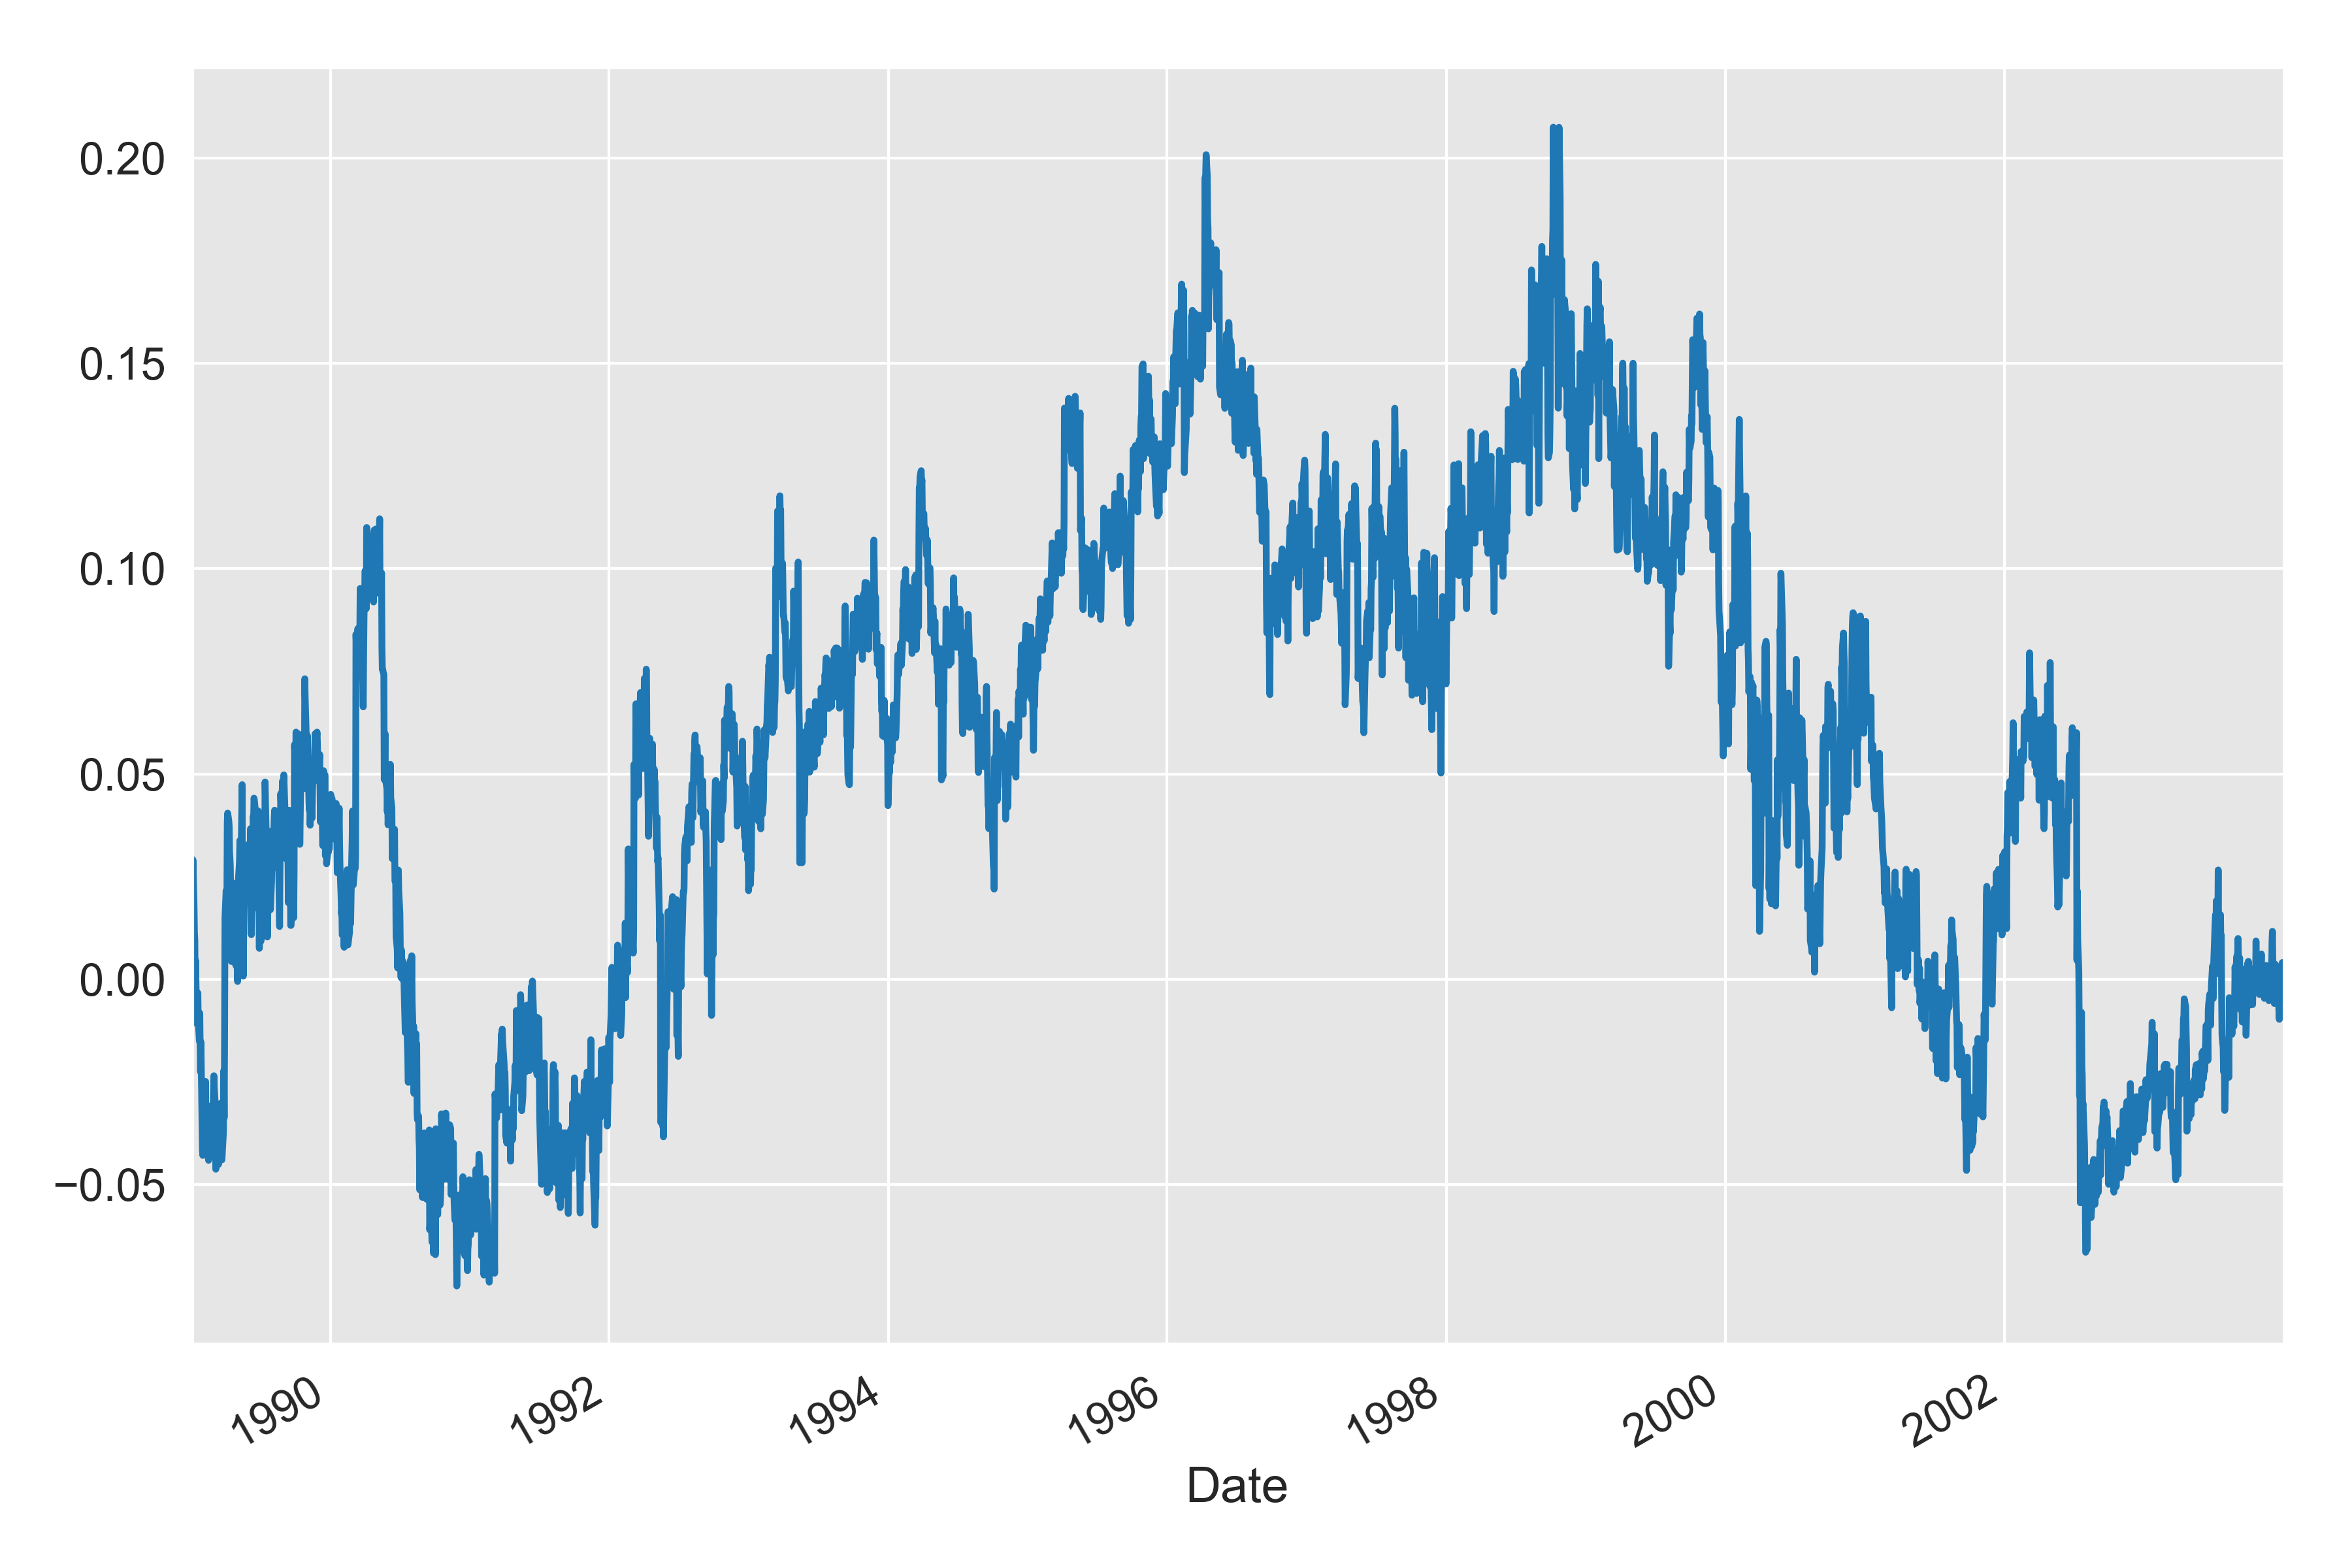
\includegraphics[width=\textwidth]{chapters/chapter_stat_ts/figures/rd_shell.png}
	\caption{Royal Dutch/Shell. \label{fig:3royal}}
	\end{figure}
	
	\begin{figure}[!ht]
	\centering
	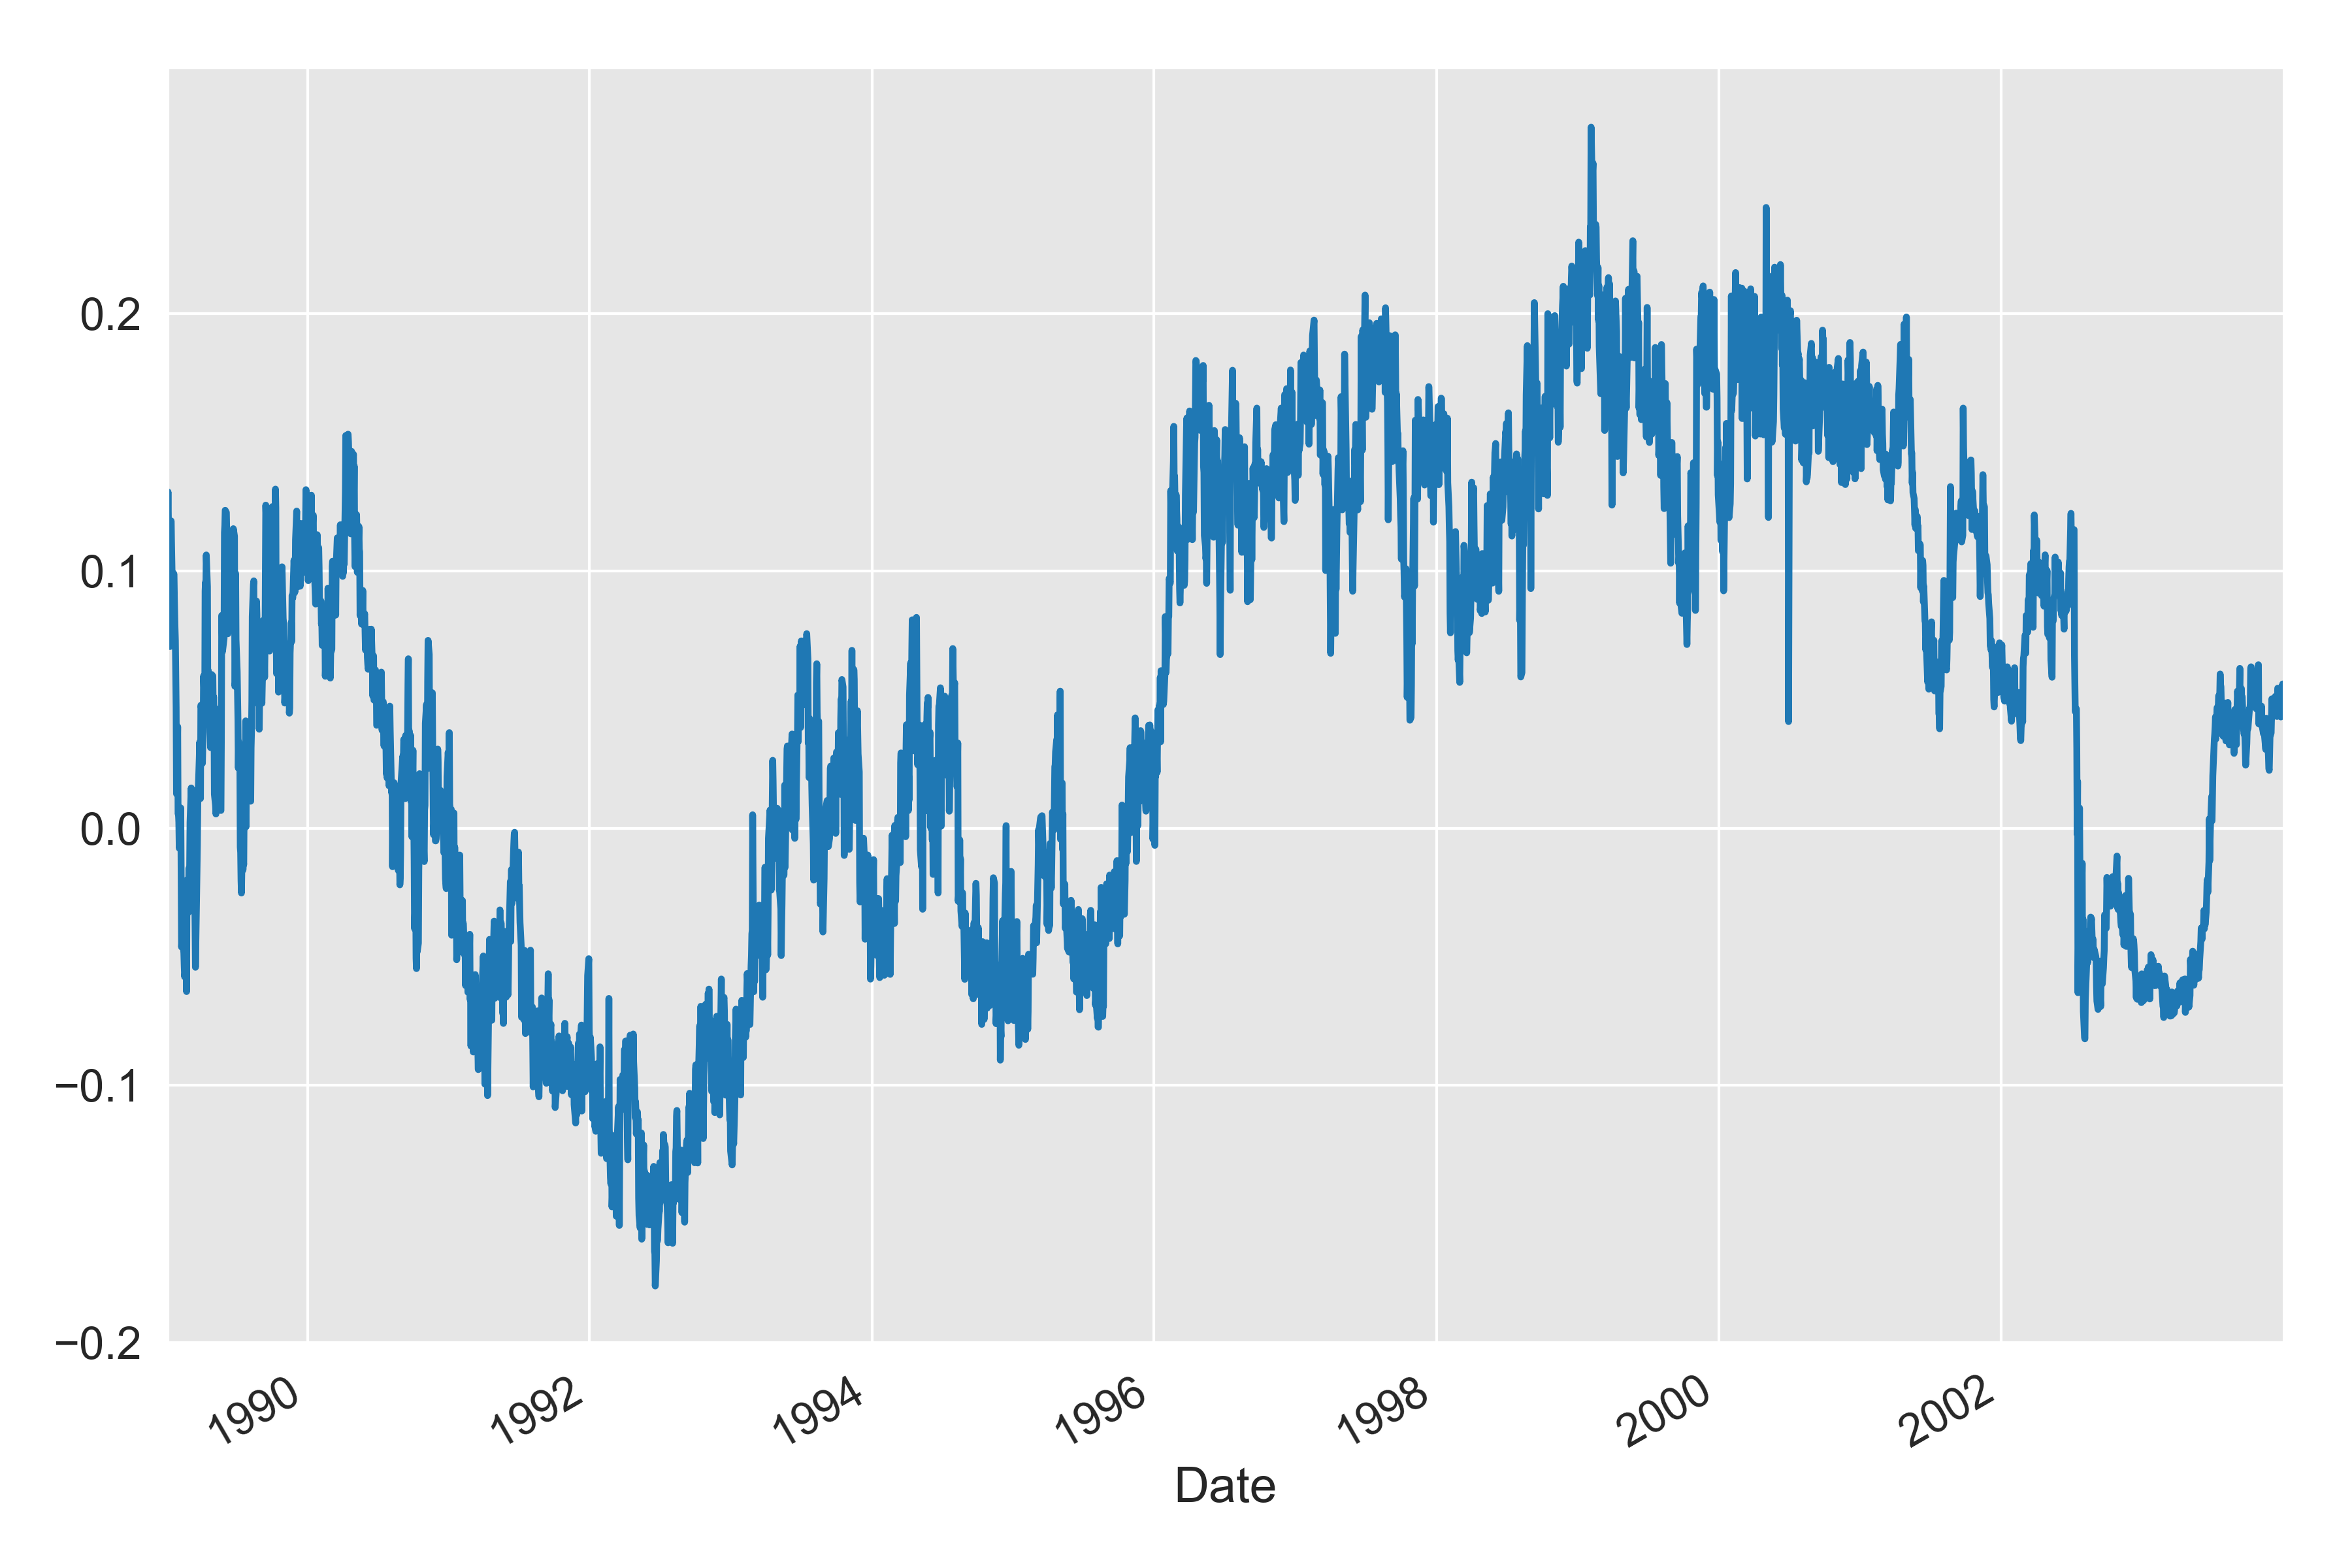
\includegraphics[width=\textwidth]{chapters/chapter_stat_ts/figures/rd_un.png}
	\caption{Unilever NV/PLC. \label{fig:3nvplc}}
	\end{figure}

The first step in developing a pairs trading strategy is selecting two or more stocks that are closer to each other. Two examples discussed here are natural-pairs as the parent company is the same and they can be called as twins. Finding such natural twins is hard in practice. As substitutes generally mature companies with long trading histories and that have similar exposure to macro factors are considered as candidates for forming pairs; usually they tend to be from the same industry. We will discuss in detail how pairs can be formed later. First we present some formal procedures for implementing the pairs trading strategy.


% Distance-Based Algorithms
\subsection{Distance-Based Algorithms}

Gatev, Goetzmann and Rouwenhorst (2006)~\cite{ggr} suggest using the distance based algorithm on normalized prices to identify the periods when the prices diverge. The normalization factor is a total cumulative returns index of the stock over the pairs formation period. Pairs are formed by computing the Euclidean distance between any two stocks and by selecting the pairs that are closer. A simple pairs trading algorithm is stated below, as illustration: \twomedskip

\noindent\fbox{%
    \parbox{\textwidth}{%
\noindent Pairs Trading Algorithm:
\begin{itemize}
\item Normalize the prices of every stock to equal unity, at the end of each calendar month, m; use the preceding 12 months as the estimation period; let $T_m$ be the number of trading days in the 12-month estimation associated with month $m$.

\item For each $t = 1,\ldots,T_m, p_t^i = \prod_{T=1}^t[1\times(1+r_T^i)]$, where $T$ is the index for all the trading days till $t$;

\item $\text{PD}_{i,j,m} = \sum_{i=1}^{T_m} \dfrac{(p_t^i - p_t^j)}{T_m}$ \hfill \break 
$\text{St.Dev PD}_{i,j,m} = \sqrt{\dfrac{1}{T_m - 1} \left(\sum_{i=1}^{T_m}[(p_t^i - p_t^j)^2 - \text{PD}_{i,j,m}]^2\right)}$

\item If price difference (PD) diverges by more than 2 St.Dev PD, buy the cheaper stock and sell the expensive one; if pairs converge at later time, unwind; if the pairs diverge but does not converge in 6 months, close the position.
\end{itemize}
        }%
} \twomedskip


Gatev et al. (2006)~\cite{ggr} study the risk and return characteristics, using daily data from 1962 to 2002, of pairs trading for stocks from various sectors. The general finding is that pairs trading is profitable in every broad sector category. In relating the excess returns to the risk factors, market, SMB, HML, momentum and reversal, it is found that the exposures are not large enough to explain the average returns of pairs trading. Thus they conclude, ``\dots pairs trading is fundamentally different from simple contrarian strategies based on reversion.''


% Co-Integration
\subsection{Co-Integration}

There is some evidence that prices are co-integrated (for a discussion on co-integration, see Chapter~\ref{ch:ch_mvts}) for the U.S. Stock market (see Bossaerts(1988)~\cite{bossaerts1988common}). If the price vector, $p_t$ is co-integrated with co-integrating rank, $r$ which imply that there are `$r$' linear combinations of $p_t$ that are weakly dependent; thus these assets can be taken as somewhat redundant and any deviation of their price from the linear combination of the other assets prices is temporary and can be expected to revert. Writing the pairs trading concept in a model form (co-integrated VAR) has several advantages. It allows us to extend pairs to triplets etc. and also the model can accommodate incorporating other factors such as other relevant indices.


A model based co-integration approach to pairs trading is elegantly presented in Tsay (2010)~\cite[Section 8-8]{tsay}. It is based on the assumption that prices follow a random walk and on the additional expectation that if two stocks have similar risk factors, they should have similar returns; writing $p_{it} = \ln(P_{it})$ and with $p_{it}$ following a random walk, $p_{it} = p_{it-1} + r_{it}$ where $r_{it}$ is the return. Thus, bivariate price series are said to be cointegrated, if there exists a linear combination, $w_t = p_{1t} - \gamma p_{2t}$ which is stationary and therefore it is mean reverting.


With the error-correlation form of the bivariate series (follows from \eqref{eqn:2Wtequiv} in Chapter~\ref{ch:ch_mvts}),
	\begin{equation} \label{eqn:errorbivar}
	\begin{bmatrix}
	p_{1t} - p_{1t-1} \\
	p_{2t} - p_{2t-1}
	\end{bmatrix}\quad
	= \begin{bmatrix} 
	\alpha_1\\ \alpha_2 
	\end{bmatrix}\quad 
	\begin{bmatrix} 
	w_{t-1} - \mu_{w}
	\end{bmatrix}\quad + 
	\begin{bmatrix} 
	a_{1t} \\ a_{2t} 
	\end{bmatrix},
	\end{equation}
where $\mu_w = E(w_t)$ is the mean of $w_t$, which is the spread between the two log prices. The quantity $w_{t-1} - \mu_w$ denotes the deviation from equilibrium, $\alpha$'s show the effect of this past deviation on the current returns and should exhibit opposite signs. Going long with one share of stock 1 and shorting $\gamma$ shares of stock 2, will result in the return of the portfolio, $r_{p,t+i} = w_{t+i} - w_t$, at time `t'. The increment does not depend on $\mu_w$.


Based on the above discussion the following strategy can be followed. \twomedskip


\fbox{%
\begin{minipage}{0.9\textwidth}
Let $\eta$ be the trading cost and $\Delta$ be the target deviation of $w_t$ from $\mu_w$ and assume $\eta < 2\Delta$.
\begin{itemize}
\item Buy a share of stock 1 and sell $\gamma$ shares of stock 2 at time t if $w_t = \mu_w - \Delta$

\item Unwind at time `$t+i$' $(i>0)$ if $w_{t+i} = \mu_w + \Delta$
\end{itemize}
Thus the return of the portfolio would be $2\Delta$ which is greater than the trading cost. 
\end{minipage}
} \twomedskip


\noindent For other modified versions of the strategy refer to Tsay (2010)~\cite[Section 8.8]{tsay}.


From a practitioner's standpoint, for testing if there is a co-integrating relationship between pairs, it is easier to use the two-step test proposed by Engle and Granger (1987)~\cite{engle1987co},
        \begin{enumerate}[(a)]
        \item Run a regression model: $p_{1t}= \alpha + \beta p_{2t} + u_t$
        \item Test if the errors, $u_t$ are stationary, via the model $u_t=\gamma + \phi u_{t-1} + a_t$, with the null hypothesis $\text{H}_0: \phi= 1$ vs  the alternative hypothesis $\text{H}_a: \phi<1$.
        \end{enumerate}
If $u_t$ is stationary, it would imply the two prices $p_{1t}$ and $p_{2t}$ are co-integrated. This test is easy to use particularly in the case of bivariate series.

	\begin{figure}[!ht]
	\centering
	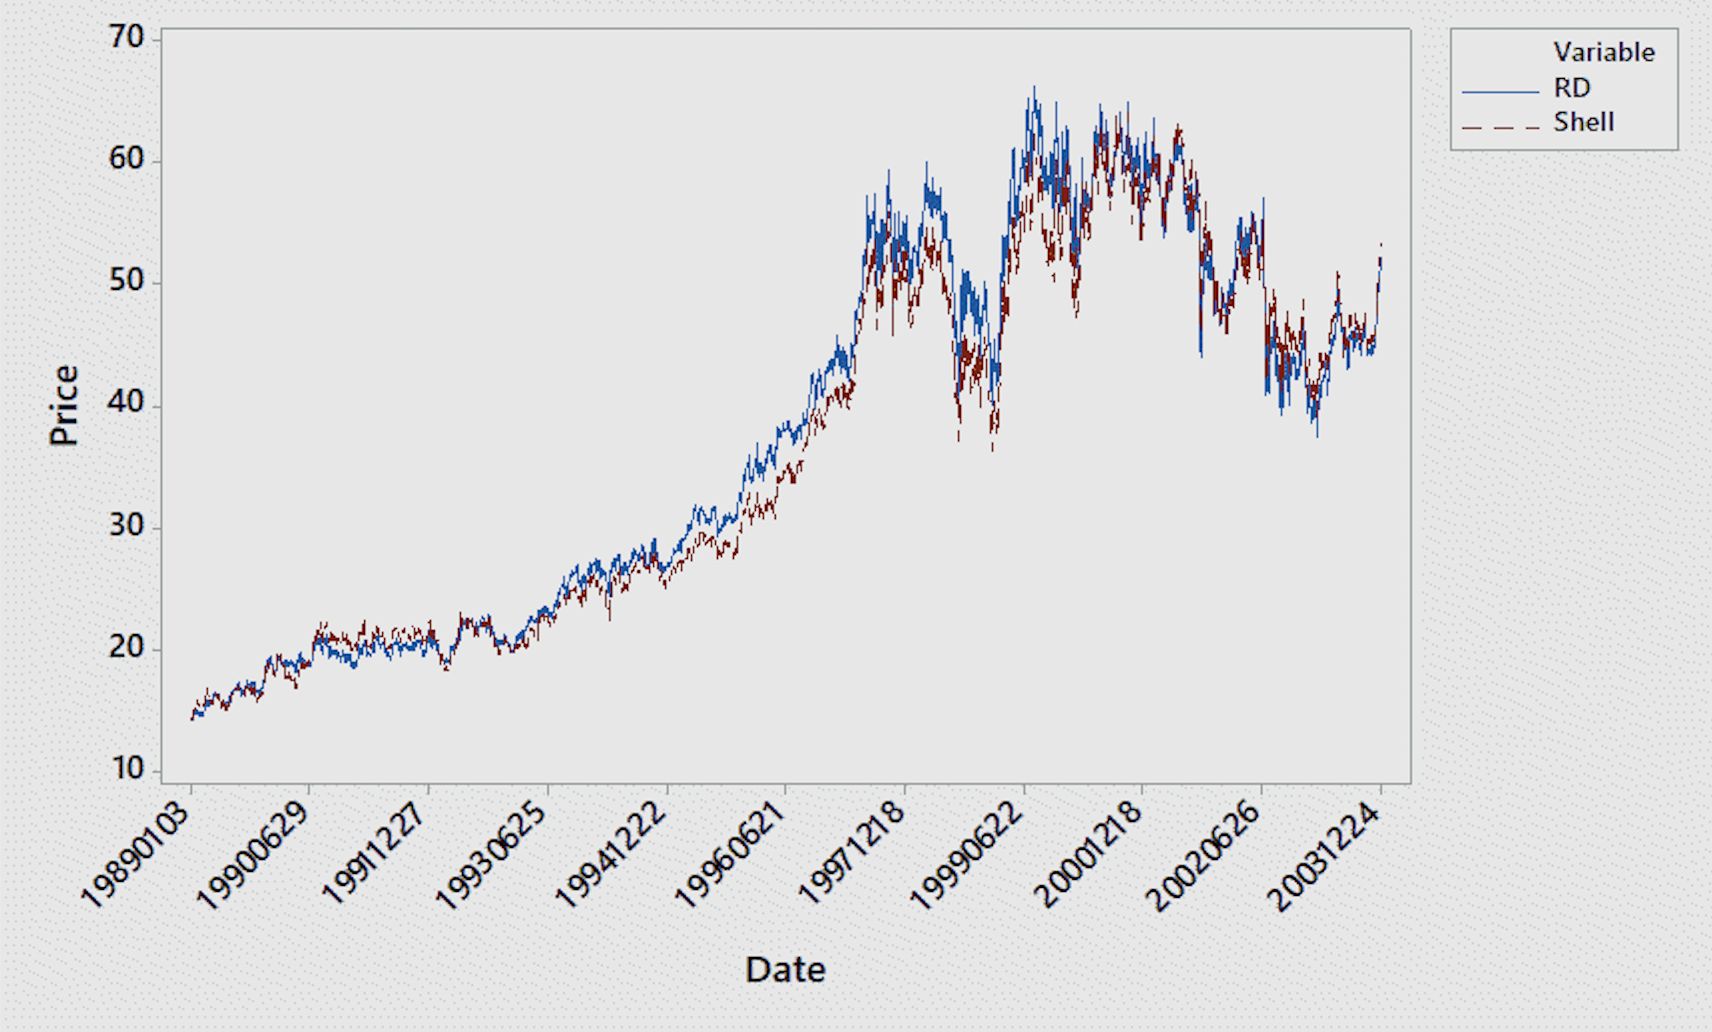
\includegraphics[width=\textwidth]{chapters/chapter_stat_ts/figures/rds.png}
	\caption{Rescaled Plot of Royal Dutch, Shell. \label{fig:rds}}
	\end{figure}
	
	\begin{figure}[!ht]
	\centering
	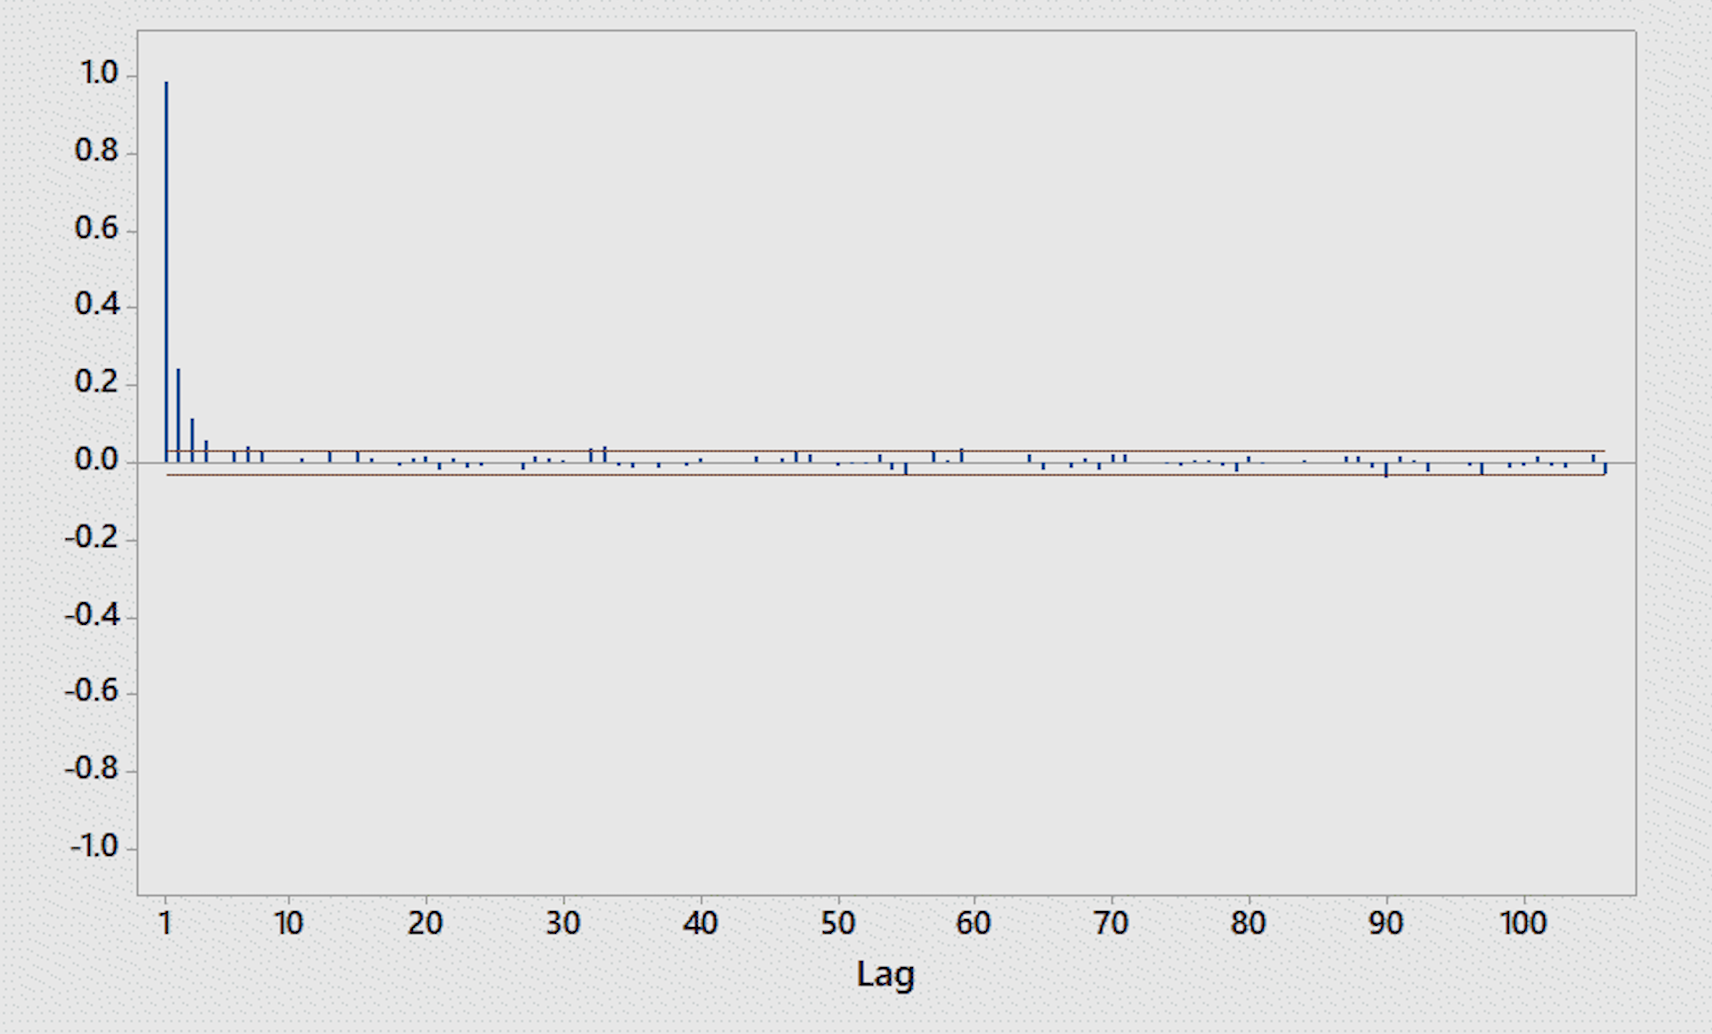
\includegraphics[width=\textwidth]{chapters/chapter_stat_ts/figures/pafresi.png}
	\caption{Partial Autocorrelation Function for RESI. \label{fig:pafresi}}
	\end{figure}
	
	\begin{figure}[!ht]
	\centering
	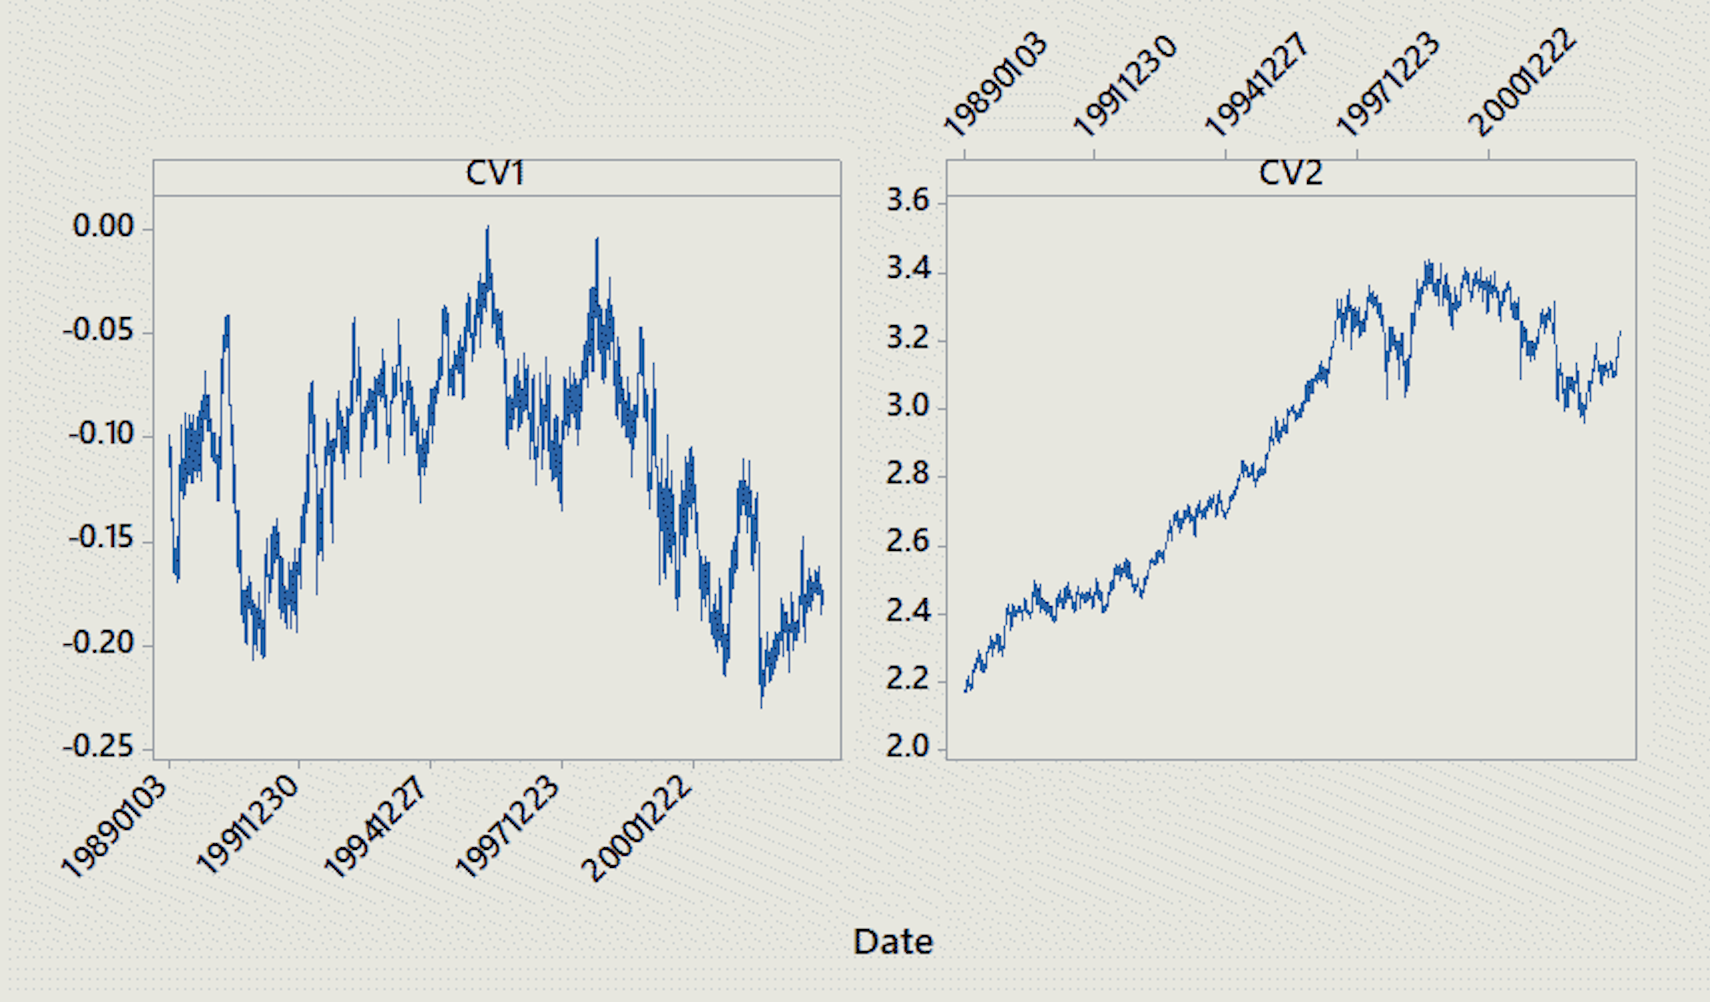
\includegraphics[width=\textwidth]{chapters/chapter_stat_ts/figures/can.png}
	\caption{Plot of Canonical Series. \label{fig:can}}
	\end{figure}


To illustrate the pairs trading strategy, we consider the Royal Dutch/Shell data. The daily data is from January 3, 1989 to December 31, 2003. The rescaled (with starting point to be the same for better visual comparison) plot is given in Figure~\ref{fig:rds}; the series are broadly aligned as expected but the gap between them at different time points is also quite evident. Let $p_{1t}$ denote the log price of Royal Dutch and let $p_{2t}$ denote the log price of Shell. Results can be summarized as follows:

\begin{enumerate}[--]
\item $\hat{p}_{1t}= -0.061^* + 1.025^* p_{2t}$, $R^2=0.988$, Durbin-Watson (DW) statistic is $0.024$ which indicates that the errors are not independent. (Recall from Chapter~\ref{chap:ch_trading_fund}, DW$\sim$2 for independent errors.)

\item Partial autocorrelation function of the estimated residual $\hat{u}_t= p_{1t} - \hat{p}_{1t}$ is given in Figure~\ref{fig:pafresi}, indicate that the residuals are stationary, probably with an AR(2) or AR(3) structure. Recall the augmented Dickey-Fuller test using the error correction form, where $v_t= u_t - u_{t-1}$ is regressed on $u_{t-1}$ and $v_{t-1}$ and $v_{t-2}$ and if the coefficient of $u_{t-1}$ is significant, it would confirm stationarity. The estimated model is, $\hat{v}_t= -0.008^* u_{t-1} - 0.273^* v_{t-1} - 0.1154^* v_{t-2}$ and the $t$-ratio that corresponds to the coefficient of $u_{t-1}$ is $-3.21$ which is significant. 

\item The error correction model \eqref{eqn:errorbivar}, which is $p_t - p_{t-1}= \Phi^* p_{t-1} + a_t$, where $p_t= (p_{1t}, p_{2t})'$ and $\Phi^* = \Phi-I$, can be shown to have rank$(\Phi^*)=1$ using the test statistic in \eqref{eqn:2negT}; the two linear combinations are $\text{CV1}= p_{1t} - 1.04 p_{2t}$ and $\text{CV2}= p_{1t} - 0.18 p_{2t}$ which are plotted in Figure~\ref{fig:can}. The first series appears to be stationary which is $w_t= \text{CV1}$ in \eqref{eqn:errorbivar}. This can be used for trading purposes using the rules discussed in the earlier part of this chapter. 
\end{enumerate}


To illustrate opportunities in pairs trading in real time, we consider the daily exchange rates between Indian rupee and U.S. dollar, GBP and Euro from December 4, 2006 to November 5, 2010. We normalize the first day's observation as unity and also note that the initial ratio is 1:1.98:1.33 in rupees for U.S. dollar, GBP and Euro respectively. From their plots in Figure~\ref{fig:rupee}, it is obvious that all three series move together until the middle of 2007, then the Euro takes off and then the U.S. dollar which is closely aligned with GBP takes off to join the Euro. For testing co-integration, one has to look at the three regimes individually. Thus tracking the co-integrating relationships over time, traders can generate profits by properly timing the swapping of currencies.

	\begin{figure}[!ht]
	\centering
	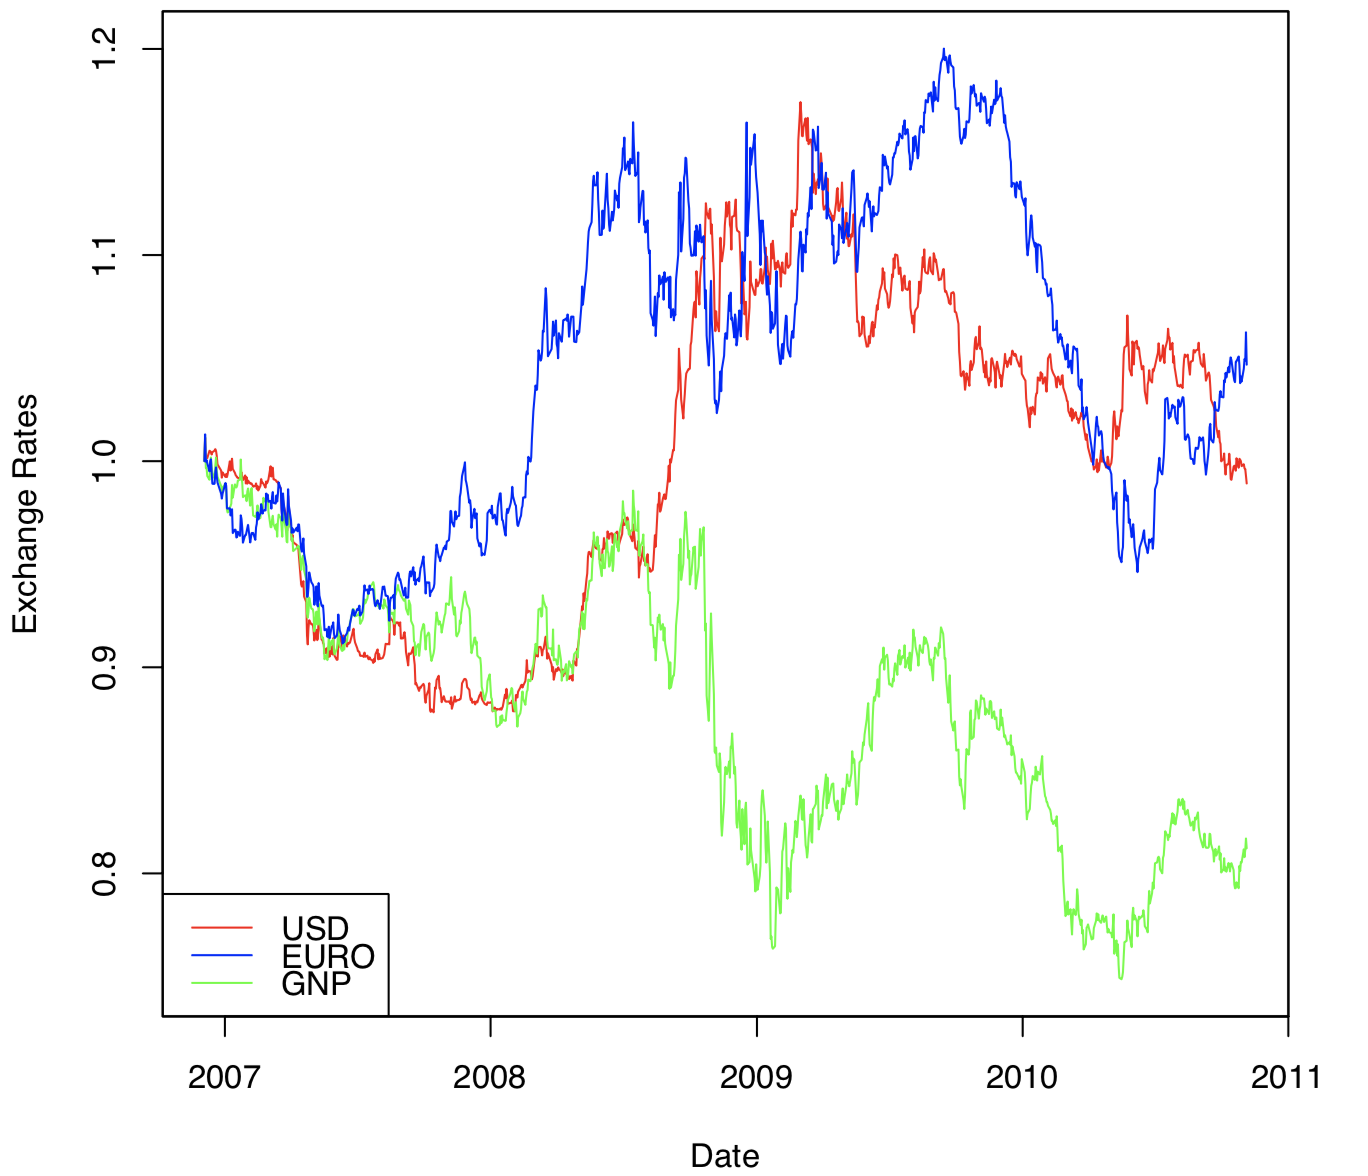
\includegraphics[width=\textwidth]{chapters/chapter_stat_ts/figures/473.png}
	\caption{Rupee Exchange Rate Data. \label{fig:rupee}}
	\end{figure}

	\begin{figure}[!ht]
	\centering
	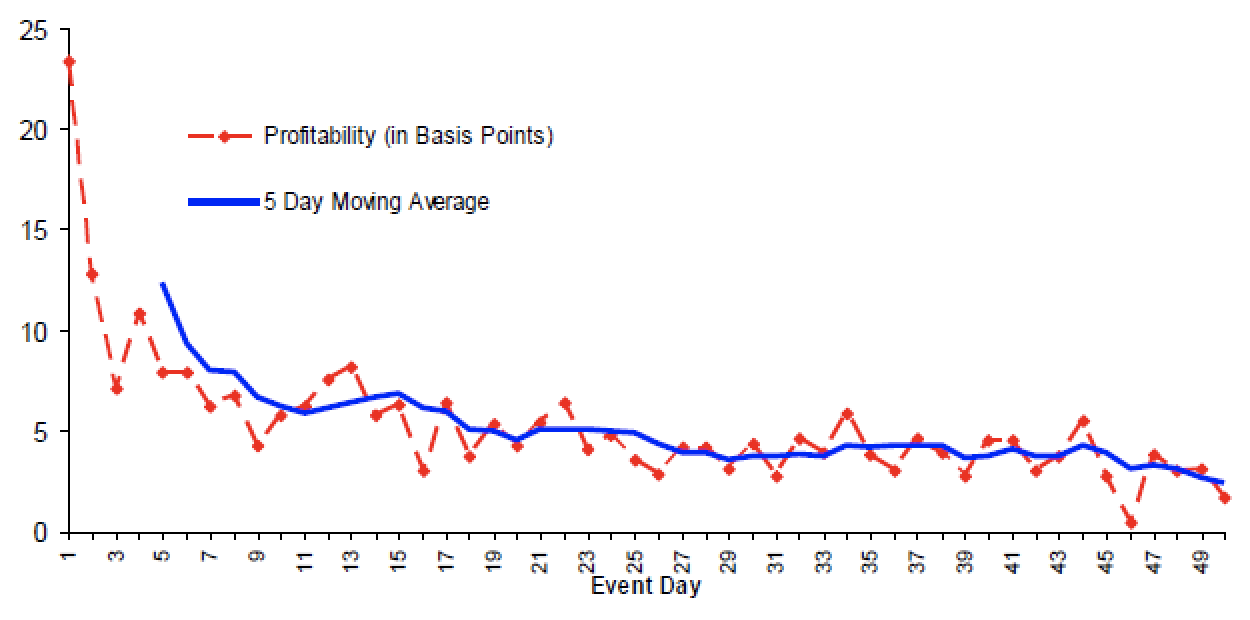
\includegraphics[width=\textwidth]{chapters/chapter_stat_ts/figures/Sec4-7Fig4.png}
	\caption{Pairs Trading Profitability in Event Time. \label{fig:pairsprofit}}
	\end{figure}

A recent study by Farago and Hjalmarsson (2018)~\cite{faragohjalm} on using co-integration method to identify pairs for trading and evaluate the strategy using Sharpe ratio. Writing the return process as $r_t= \mu + u_t$ and $u_t$-process capturing the autocorrelation in the returns, the price process $\beta_t$ is decomposed into a deterministic trending component (equivalent to a drift), a non-stationary martingale component and a transitory noise component. The co-integration process generally elimination both the trending and martingale components and thus leaving the convergence of the pairs to mainly transitory component. The co-integration of any two stocks in the market which implies long-run relationships is not likely to occur.


% Some General Comments
\subsection{Some General Comments}

\noindent\textbf{Finding Pairs:} An alternative approach is to use fundamentals of the firms to select two stocks that have similar risk factor exposures. Based on Asset Pricing Theory (APT) model,
	\begin{equation}
	r_{it} - r_{ft} = \alpha_i + \beta'_if_t + a_{it},
	\end{equation}
where $r_{ft}$ is the risk-free rate and $f_t$ are the factor scores. Now collect the coefficient vector $\hat{\theta}_i' = (\hat{\alpha}_i, \hat{\beta}_i)'$ for $i = 1, 2, \ldots, N$ assets under consideration and form a standardized distance measure,
	\begin{equation} \label{eq:dijsquaredcov}
	d_{ij}^2 = \hat{\theta}_i' \cov^{-1}(\hat{\theta}_i)\hat{\theta}_i
	\end{equation}
and select pairs with the smaller distance. This can be expected to result in similar assets after adjusting for the risk factors. Generally the factors tend to vary much more slowly than the excess returns, $r_{it} - r_{ft}$, the distance based on $\hat{\theta}_i$ tends to move slower than short-term price movements. Recent studies confirm that the simple Euclidean distance-based pairing may be inadequate. Do and Faff (2010)~\cite{do2010does} suggest adding two additional metrics: industry homogeneity and the frequency of the historical reversal in the price spread; the measure in \eqref{eq:dijsquaredcov} can accommodate that easily. \twomedskip


\noindent\textbf{High Frequency Equity Pairs Trading:} While there is evidence of the profitability of pairs trading strategies at lower frequencies, not much is known in academia (but quite known in practice) about high frequency intra-day pairs trading. Bowen, Hutchinson and O'Sullivan (2010)~\cite{bho} consider data from the London Stock Exchange for the most liquid stocks, the constituents of the index FTSE100. The duration is divided into a formation period, that is used to identify pairs of stocks that move together, and a trading period when the actual transactions occur. The distance based criteria using normalized prices is used to identify the top pairs during the formation period. As any other strategy, pairs trading profits are affected by transaction costs, and this becomes more acute as trading frequency increases. Results appear to be also quite sensitive to the speed of execution, as excess returns disappear quickly if delay in execution is greater than one period. The majority of profits seem to occur in the first and last hour of trading, when relatively larger volatility and liquidity occur.


Although pairs trading has been used extensively by traders, it also has its limits. In a recent study, Engelberg, Gao, Jagannathan (2009)~\cite{engelberg2009anatomy} demonstrate that the opportunities for medium frequency pairs trading are not many and profits opportunities might vanish within a few days (see Figure~\ref{fig:pairsprofit}). Scruggs (2007)~\cite{scruggs} attributes the demise of Long-Term Capital Management to the hedge fund overconfidence in the strategy and their undue bet sizes compared to other market participants.


% Practical Considerations
\subsection{Practical Considerations \label{s:pract_consid}}

After identifying a potential pairs strategy via co-integration testing for instance, traders need to pay particular attention to the expected profitability of the strategy once real-life trading frictions have been taken into consideration. In practice, a significant portion of potential pairs trading strategies experience negative P\&L in production due to large execution slippage, whether originating from aggressive hedging at trade initiation, or position closing out.


When back testing a pairs strategy, one of the immediate cost that might render the strategy unprofitable is the spread cost. In other words, how much will it cost to extract liquidity when the signal triggers, in particular if the signal is too short-lived to allow for sourcing liquidity passively via limit order book posting. For intraday pairs trading it is also valuable to analyze if there is any asymmetry of cost between the initiation trade and the unwind trade. Often time, it is not uncommon to witness significantly higher exit costs once the market has normalized following a short-lived entry trade opportunity. 


The individual instrument's microstructure also plays an important role in the strategy profitability. For instance long queue names  (instruments for which the top of book liquidity is large in comparison to daily volume)  are harder to trade because the time it takes for an order to reach the top of the queue and trade passively is generally larger than the time that is acceptable for the strategy to mitigate its legging risk.\footnote{Legging risk can be defined as the risk of not being able to fill timely a particular leg of a pair strategy at the required price.} As a result, most of the executions on the leg that displays a long queue will end up having to pay the full spread to be executed. 


As an example, when computing the spread ratio between two instruments using the market midpoint, one might be led to believe that the ratio is currently above $2\sigma$ of its distribution, warranting to initiate a trade. However, when considering the size of the spread and amount of the quoted volume on the passive side at the top of the book, it is not impossible that the realized ratio when crossing the spread is only a $0.5\sigma$ event, while getting a passive execution when quoting at the end of a long queue would represent a $5\sigma$ event that one shouldn't expect to realistically happen. These anecdotal examples give an idea of what practitioners should pay particular attention to when designing their strategies. Below, we mention a non-exhaustive list of implementation challenges also worth considering:


\begin{itemize}
\item \textbf{Difference in liquidity between the two legs:} Usually the selected pair has a slower moving leg and a faster moving one. This means that, in practice, one of the instruments might be ticking faster, thereby having a greater influence on the moves of the measured ratio. Additionally, faster ticking instruments also tend to have narrower spreads, meaning that in absence of control, the instrument the most likely to trigger a trade is also the one that is the cheapest to transact, forcing the strategy to then rapidly hedge out its exposure by paying the larger spread on the slowest ticking leg. One way of handling this situation is, for instance, to only let the strategy quote on the slow moving leg as long as it is ``in ratio'', and then only trigger the aggressive spread-crossing hedge trade if and when the passive leg receives a fill. 

\item \textbf{Rounding/tick size granularity:} While in theory it is possible to come up with a signal threshold that is as granular as desired, in practice the step increment of the signal might be constrained by the microstructure of the instruments traded. Most exchanges globally impose a minimum tick size increment that can vary based on the liquidity of the instrument. Here too, all things being equal, a practical approach would be to quote on the instrument which constrained tick size contributes the most to the ratio moves, and only trigger the aggressive spread-crossing hedge trade if and when the most constrained tick size leg receives a fill. 

\item \textbf{Signal stability:} As a result of both the difference in liquidity between long and short legs, and the potential frictions induced by the instruments microstructure described above, it is not uncommon for the signal to jump around the trigger ratio frequently. Trading in and out on each signal crossing of the pre-determined ratio would incur large transaction costs that would render many strategies unprofitable. To address this issue, a common approach is to define two different thresholds sufficiently apart for entering and exiting the trade so that signal noise does not trigger excess in and out trading. It is also possible to enforce a minimum holding duration to prevent the stop loss signal to trigger just due to local noise around the ratio threshold. 

\item \textbf{Time of day:} In the first 15 to 30 minutes after a market opens, many instruments have significantly wider bid-ask spreads while price discovery sets in after a night of information accumulation and no possible trading. If this significant difference in transaction costs is not properly accounted for, the trades initiated during that period can have an impact on the overall profitability of the strategy.

\item \textbf{Market asynchronicity:} While pairs are usually constructed between instruments trading concomitantly, it is also possible to construct pairs strategies with instruments from different markets. For instance, a pair between a US and a Japanese stock. This raises an additional challenge, which is: how to assess the theoretical value on an instrument that is not currently traded? Practitioners commonly address this issue by first modeling the relationship between the instruments daily time series, and then inferring its stability at more granular frequencies. The common risk can be hedged with a market wide instrument such as an index future, and be unwound overnight when the second leg is entered, thereby limiting unwanted exposure to market risk.

\item \textbf{Traditional Index Arb / ETF Arb:} When trading a pairs strategy between a composite instrument (Index, ETF, \dots) and its constituents, the fast and efficient nature of electronic markets might render trading opportunities too small to be exploited profitably across all instruments. In particular if the number of constituents is quite large, obtaining passive fills on most of them within a reasonable time frame is not a realistic assumption. As a result, traders can implement partial replication strategies whereby they only trade an optimized tracking basket of the instruments that allow for the best replication under some liquidity and cost assumptions (spread size, top of book size, \dots). 

\item \textbf{Local market idiosyncrasies:} For instance, in Japan, sector classification (which is often used as a starting point for pairs selection or as a way to avoid picking names that would have spurious autocorrelation) does not match international sector classification one-to-one. Local market participants rely on the 33 TOPIX sectors that have a closer fit to the actual structure of the Japanese economy than the commonly used 11 GICS\textsuperscript\textregistered sectors.

\item \textbf{Coupling market making and pairs trading strategies:} One possible approach to long queue and wide spread instruments pairs trading is to use a market making strategy to first gain queue priority in the longest queue name and achieve a certain child order density in the order book at regular volume-time intervals. For example, if only one of the instruments has a long queue, as long as the pairs strategy ratio is below the trigger threshold, the market making strategy can earn the spread on the long queue instrument while staying out of the market on the other instrument. When the ratio reaches the threshold, one can cancel the child orders created on the opposite side of the book by the market making strategy and only keep the ones on the side relevant to the pairs strategy. These orders, placed over time while market making, should already have accrued some queue priority, which will increase the probability of receiving a passive fill once the ratio is favorable. Then, the pairs strategy is able to trade aggressively the liquid leg as soon as the passive fill is received. Based on the liquidity and microstructure of the instruments in the pairs strategy, different equivalent strategies can be combined to achieve higher profitability.
\end{itemize}



% Cross-Sectional Momentum Strategies
\section{Cross-Sectional Momentum Strategies}

The trading strategies discussed thus far depend exclusively on the existence of time-series patterns in returns or on the relationships between returns and the risk factors. Time series strategies generally exploit the fact that stock prices may not follow random walks, at least in the short run. Even if prices follow random walk, it has been shown that strategies based on past performance contain a cross-sectional component that can be favorably exploited. For instance, momentum strategies demonstrate that the repeated purchase of past winners from the proceeds of the sale of losers can result in profits. This is equivalent to buying securities that have high average returns at the expense of securities that yield low returns on average. Therefore if there is some cross-sectional variance in the mean returns of the securities in the universe, a momentum strategy is profitable. On the other hand, a contrarian strategy will not be profitable even when the prices follow random walk. For the demonstration of the rules of the momentum strategy in the low frequency setting, refer to Jegadeesh and Titman (1993)~\cite{JeTit1993}, 2002~\cite{JeTit}) and Conrad and Kaul (1998)~\cite{conrad1998}.


To better understand the sources of profit from a momentum strategy Lo and MacKinlay (1990)~\cite{lo1990} decompose the profit function into three components. We will follow the set-up as presented in Lewellen (2002)~\cite{lew2002}. Let $r_{i,t-1}^k$ be the asset $i$'s, `$k$' month return ending in `$t-1$' and let $r_{m,t-1}^k$ be the return from the equal-weighted (market) index's `$k$' month return ending in `$t-1$'. The allocation scheme over `$N$' assets under the momentum strategy is,
	\begin{equation} \label{eqn:witkrdiff}
	w_{i,t}^k= \frac{1}{N} (r_{i,t-1}^k - r_{m,t-1}^k), \quad i= 1,\ldots, N.
	\end{equation}
For ease of interpretation, $w_{i,t}^k = w_{i,t}$ and focus on only one previous month's return for allocation; let $r_t$ be a $N \times 1$ vector of returns, with the mean return $\mu = E(r_t)$ and $\Omega = E[(r_{t-1} - \mu)(r_t - \mu)']$ the autocovariance matrix of returns. Let $w_t$ be $N \times 1$ vector of weights, $w_{it}$; the portfolio return for month `t' is $\pi_t = w_t'r_t$. It is easy to show
	\begin{equation} \label{eqn:epitomega}
	\begin{split}
	E(\pi_t)&= \frac{1}{N}\, E\left[\sum_i r_{i,t-1} \cdot r_{it} \right] - \frac{1}{N} E\left[r_{m,t-1} \cdot \sum_i r_{it} \right] \\
	&= \frac{1}{N}\sum_i (\rho_i + \mu_i^2) - (\rho_m + \mu_m^2),
	\end{split}
	\end{equation}
where $\rho_i$ and $\rho_m$ are lag 1 autocovariances of asset `$i$' and the equal weighted index. Note that the average autocovariance is $\text{tr}(\Omega)/N$ and the autocovariance for the market as a whole is $(1' \Omega 1)/N^2$. The $\text{tr}(\Omega)$ denotes the sum of the diagonal elements of $N \times N$ matrix $\Omega$; recall that the diagonal elements are the autocovariance, $\rho_i$, of individual stocks. Hence \eqref{eqn:epitomega} can be written as,
	\begin{equation} \label{eqn:3epi}
	E(\pi_t) = \left(\frac{N-1}{N^2}\right)\cdot \text{tr}(\Omega) + \frac{1}{N^2} [\text{tr}(\Omega) - 1' \Omega 1] + \sigma_{\mu}^2.
	\end{equation}
The three terms in \eqref{eqn:3epi} precisely identify three sources why positive profits can occur (see Lo and Mackinlay (1990)~\cite{lo1990}):


\begin{itemize}
\item Stock returns are positively autocorrelated, so each stock's past return predicts high future return.
\item Stock returns are negatively correlated with the lagged returns on other stocks, so poor performance of some stocks predicts high returns for others
\item Some stocks have simply high unconditional mean returns relative to other stocks.
\end{itemize}


The finance literature is replete with empirical verifications of the momentum strategy. However, the analytical decomposition in \eqref{eqn:3epi} is not informative about the economic sources of momentum. Why the momentum strategy works has been attributed to various theories. The literature argues that firm-specific returns drive momentum. Firm-specific returns can be persistent because investors under-react to firm-specific news or stock returns covary strongly due to a common influence of a macro factor. Lewellan (2002)~\cite{lew2002} shows that the Size and B/M portfolios also exhibit strong momentum; as these portfolios are well-diversified, their returns reflect systematic risk and therefore macroeconomic factors must be responsible for the momentum. Hvidkjaer (2006)~\cite{hvid2006} suggests that momentum could be partly driven by the behavior of small traders who under-react initially, followed by delayed reaction to buying and selling pressures. The trading pressure tends to translate into price pressures that affect the trading behavior of the small traders.


Although cross-sectional momentum is widely documented, among the three components in \eqref{eqn:3epi}, time series momentum as represented by the first term tends to dominate for every liquid instrument in a study of fifty-eight instruments spread over a variety of asset classes, equity index, currency, commodity and bond futures. Moskowitz, Ooi and Pedersen (2012)~\cite{mos2012} show that the autocovariance term, $\tr(\Omega)/N$ is the dominant factor, particularly in foreign exchange and equity markets. To make meaningful comparison across asset classes, the excess returns are scaled by their ex-ante volatilities and the following models are estimated for predicting price continuation and reversal:
	\begin{equation} \label{eqn:pricecontrev1}
	\frac{r_t^s}{\sigma_{t-1}^s} = \alpha + \beta_h \dfrac{r_{t-h}^s}{\sigma_{t-h-1}^s} + \varepsilon_t^s
	\end{equation}
and
	\begin{equation} \label{eqn:pricecontrev2}
	\frac{r_t^s}{\sigma_{t-1}^s} = \alpha + \beta_h \sgn(r_{t-h}^s) + \varepsilon_t^s,
	\end{equation}
where $h= 1,2, \ldots, 60$ months and the ex-ante annualized variance $\sigma_t^2$ is calculated as follows:
	\begin{equation} \label{eqn:pricecontrev3}
	\sigma_t^2 = 261 \sum_{i=0}^\infty (1 - \delta)\,\delta^i \,(r_{t-i} - \overline{r}_t)^2.
	\end{equation}
Here the weights $\delta^i (1 - \delta)$ add up to one, $\overline{r}_t$ is the exponentially weighted average return computed in a similar fashion. The exponential smoothing parameter is chosen to be $\sum(1 - \delta)\, \delta^i = \frac{\delta}{1 - \delta} = 60$ days. Using $\sigma_{t-1}$ in \eqref{eqn:pricecontrev1} and \eqref{eqn:pricecontrev2} avoids the look-ahead bias.\footnote{This occurs if data otherwise not available at the time of study is used in simulation or developing strategies.}


We can also investigate the profitability of strategies based on time series momentum with varying look-back period ($k$) and holding period ($h$). The trading strategy is that if the excess return over the past $k$ months is positive, go long or otherwise go short. The position size is taken to be, $1/\sigma_{t-1}^s$, inversely proportional to the ex-ante volatility of the instruments, `$s$'. With this choice it is argued that it will be easier to aggregate the outcome of the strategies across instruments with different volatilities and it will also lead to somewhat stable time series. For each trading strategy $(k, h)$, a single time series of returns, $r_t^{\text{TSMOM}(k,h)}$, which is the average return across all portfolios active at time, `$t$' is computed. To evaluate the overall value of the time series momentum strategies, the returns are adjusted for possible risk factors:
	\begin{equation} \label{eqn:tsmom}
	\begin{split}
	r_t^{\text{TSMOM}(k,h)}&= \alpha + \beta_1 \text{MKT}_t + \beta_2 \text{BOND}_t + \beta_3 \text{GSCI}_t + \beta_4 \text{SMB}_t \\
	&=  + \beta_5 \text{HML}_t + \beta_6 \text{UMD}_t + a_t,
	\end{split}
	\end{equation}
where $\text{MKT}_t$ is the excess return on the MSCI World index, $\text{BOND}_t$ is Barclay's Aggregate Bond Index, $\text{GSCI}_t$ is S\&P GSCI commodity index and the others are Fama-French factors for the size, value and cross-sectional momentum premiums.


Using monthly data spanning January 1985 to December 2009, Moskowitz et al. (2012)~\cite{mos2012} find that the time series momentum strategies provide additional returns over and above a passive buy and hold strategy. They also show that the model \eqref{eqn:tsmom} results in a large and significant alpha. The analysis also illustrates that speculators are likely to benefit from trend following at the expense of hedgers. The time series momentum appears to last about a year and then begins to reverse. It is shown that the momentum strategies remain profitable even after adjusting for price impact induced by trading. Although the trading decisions are done at a macro level, the actual trading takes place at a micro level. The price impact (see Chapter~\ref{chap:ch_mi_models}) is the impact of the current trade on the subsequent trades. 


The role of trading volume in explaining the results of momentum strategies is studied in Lee and Swaminathan (2000)~\cite{lee2000}. They find that, in equilibrium, both price and volume are simultaneously determined and thus both can exhibit momentum. In addition to the decile classification based on the past returns, the universe of stocks was further divided into three volume size categories, yielding thirty groups. The study provides evidence that low volume stocks tend to be under-valued by the market. Thus investor expectations affect not only a stock return but also its trading volume. High volume firms generally earn lower future returns. The general notion that volume fuels momentum is not supported but is true for losers and ``it helps information ``diffusion'' only for winners.''


It is worth mentioning that while most documented applications of the momentum strategy are in equity markets, there is a growing academic interest in their use in foreign exchange (FX) markets. The FX markets were traditionally cited as markets where technical rules such as trend following have been successful. But studies such as Menkhoff, Sarno, Schemeling and Schrimpf (2012)~\cite{menkhoff2012} have explored the cross-sectional momentum and have demonstrated their profitability (up to 10\%) in FX markets. The momentum portfolios in FX markets are observed to be skewed toward minor currencies but trading them have somewhat higher transaction costs. The base currency returns, $r_t= \ln(S_t) - \ln(S_{t-1})$ where $S_t$ is the spot exchange rate, and the interest-adjusted return, where $F_{t-1}$ is the future price at $t$-1,
	\begin{equation}
	\begin{split}
	r_t^* &= \ln(S_t) - \ln(F_{t-1}) \\
	&= \ln(S_t) - \ln(S_{t-1}) + \ln(S_{t-1}) - \ln(F_{t-1}) \\
	&\sim r_t + \dfrac{r_f - r_d}{12},
	\end{split}
	\end{equation}
which is the sum of pure currency appreciation and the return due to interest rate appreciation. Here $r_f$ is the foreign interest rate and $r_d$ is the domestic interest rate; See Okunev and White (2003)~\cite{okunev2003} for the details of this decomposition. It is found that the profitability is clearly originating from spot rate changes themselves and not necessarily driven by the interest rate differential.


In the equity markets, it is argued that momentum strategies are successful because of slow information processing and investor overreaction. However FX markets are dominated by professionals and thus any information should be impounded in the FX rate almost instantaneously. But if the portfolios are mostly made up with minor currencies, they are likely to exhibit higher volatility, higher country risk and higher interest-rate changes, thus imposing effective limits to arbitrage. It is further observed that the cross-section based currency momentum is not related to benchmark technical trading strategies and even after adjusting for them, the cross-sectional momentum profits are found to be higher. \twomedskip


\noindent \textbf{Other Sorting Criteria:} \twomedskip


The classical momentum studies described above tend to focus on stratifying the stocks in ten deciles based on the past average returns. Han, Yang and Zhou (2013)~\cite{hanyangzhou} suggest sorting based on volatility which reflects the information uncertainty. Other sorting criteria may include credit rating, distance to default, etc.. After sorting by volatilities, the decile portfolios are formed. The strategy then is to use the moving average based rule (see Section~\ref{s:trading_rules_tad}) as follows: if the price is above the moving average, buy or continue to hold or else invest in a risk-free asset. The performance of this strategy is then compared with buy and hold method. It is shown that this strategy results in positive returns and generally these returns increase with the volatility. If the returns are further adjusted for market risk (CAPM) and Fama-French factors, the average returns are greater and increase with the volatility levels. Two items of note here: as the returns are adjusted for the risk factors, they are likely to result in fewer trading opportunities as these models become more restrictive; if results are not adjusted for transaction costs and buying and selling a portfolio of stocks can be expensive and so the results may be too optimistic.  



% Multiple Indicators and Boosting Methods
\section{Multiple Indicators and Boosting Methods \label{sec:multindboostmeth}}

In developing models that capture the main features of the data, it must be noted that there are no unique models. Thus they yield different forecasts. It is well-known in the forecasting literature that a combined forecast generally does perform overall better than the individual forecasts. If there are `$T$' models and thus `$T$' forecasts, $\hat{f}_1,\ldots, \hat{f}_T$, how do we combine them to get a single forecast? Because these are all based on the same data, the estimates are likely to be correlated, resulting in a covariance matrix, $\hat{\Sigma}_f$. Three estimates that are proposed in the literature are:

	\begin{table}[!ht]
	\caption{Three proposed estimates}
	\begin{tabular}{l l r}
	\textbf{Weighted Estimator 1: \hskip 1mm} & $\hat{f}_{w_1}=\hat{f}' \hat{\Sigma}_f^{-1} \hat{f}$ \\
	\textbf{Weighted Estimator 2: \hskip 1mm} & $\hat{f}_{w_2} = \hat{f}' (\text{diag}\hat{\Sigma}_f)^{-1} \hat{f}$ \\
	\textbf{Simple Average Estimator: \hskip 1mm} & $\sum_{i=1}^T \frac{\hat{f}_i}{T}$ 
	 \end{tabular}
	 \end{table}

\noindent Due to the uncertainty in the estimation of $\Sigma_f$, especially in regime changes that may result in large estimation error, the simple average estimator is sometimes advocated. In the context of modeling the asset prices the elements of $\Sigma_f$ represent how well the methods do in forecasting. In order to use the above weighted estimators we need to keep track of the performance of the individual forecasting methods and in principle, the methods that yield inferior forecasts would get less weight. But a question about the span of their performance, whether to use more recent versus past data, remains open. \twomedskip


\noindent \textbf{Ensemble Learning} \twomedskip


As mentioned, the idea of combining multiple forecasts (classifiers) into a single one is a longstanding goal of many decision-makers. This is especially important when methods that are successful in different regimes are complementary. There are two types of ensemble methods, bagging and boosting that we discuss here. Suppose the goal is to determine if we want to enter the market or not based on the information available at that time. It is somewhat easier to come up with simple rules but is harder to find a rule that has high accuracy. Under boosting, we study how to combine the simple rules uniformly into a `stronger' rule. It is suggested to focus on examples that are hardest to forecast by simple rules and take a weighted majority of these rules to come up with a stronger rule.


To motivate, we will assume that we want to determine whether the price of an asset will go up or down. Under the random walk model, the error in guessing randomly is 0.5. But any rule should result in an error less than 0.5. We begin with a training set, $S=\{ (x_i,y_i), i=1,2, \ldots n\}$ where $x_i$ is the information and $y_i$ is a binary variable that indicates whether to enter the market or not. Assume that there are `$T$' rules, $h_t(x)$ are the classifiers and $D_t$ is the distribution over the training set with the error,
	\begin{equation}
	\text{err}_D(h)=Pr_{(x,y) \sim D}(h(x) \neq y).
	\end{equation}
The rule $h_t$ is supposed to have error $\text{err}_{D_t}(h_t)$ with respect to `$D_t$'. \twomedskip


\noindent The boosting algorithm works as follows:

        \begin{table*}[!ht]
        \begin{tabular}{r l r}
        \textbf{Initialize:} & $D_t(i)=\frac{1}{n}$ for all $i$  \\
        \textbf{Iterate:} & $D_{t+1}(i)=\frac{D_t(i)}{z_t} \cdot \text{exp}[-\alpha_t y_i h_t(x_i)]$, \\
        & where $\alpha_t=\frac{1}{2}\text{ln} \left( \frac{1-\text{err}_{D_t}(h_t)}{\text{err}_{D_t}(h_t)} \right), z_t=$ normalizing constant \\
        \textbf{Stopping Time:} & Stop when the error in (1) on a validation data set does \\
        & not improve \\
        \textbf{Final Rule:} & $\text{Sign}(\sum_{t=1}^T \alpha_t h_t(x))$  \\
        \end{tabular}
        \end{table*}
 
 
 It is possible that overfitting can happen with boosting; its performance clearly depends upon how well the two decisions (enter or not enter) are clearly separated based on the past data. The use of kernels can improve local separability. It is also important to optimally extract features, $x$, that can be discriminating between the two options for $y$. The main advantage of ensembles of different rules is that it is not likely that all rules will make the same error. The algorithm described above is known as, ``adaptive boosting algorithm (AdBoost)'' is by Freund and Schapire (1995, 1996,1997)~\cite{freund1995decision,freund1996experiments,freund1997decision} and it automatically ``adapts'' to the data at hand. If $t^{th}$ classifier $h_t(x)$ is parameterized and the overall predictor takes the form
	\begin{equation}
	h(x)=\text{Sign} \left( \sum_{t=1}^T \alpha_t \text{Sign}(w^{(t)}x+b^{(t)}) \right)
	\end{equation}
is a two-layer neural network with `$T$' hidden units. One can see the identical underlying nature of the structure between neural network and boosting algorithm.


The idea of bagging comes from training the rules on multiple data sets that supposedly have similar structure. The multiple data sets are obtained by bootstrap  resampling. The bootstrap data sets are not likely to be too similar. For the data on asset prices, which are represented by an AR(1) model with the coefficient close to one, the asymptotic distribution of the sample estimate of the coefficient is non-normal. So the bootstrap samples are also useful to construct the appropriate sampling variance. The bootstrap samples are created by resampling the innovations or empirical residuals. From the single data set, $S$ we create `$M$' bootstrapped samples, $S_1, \ldots, S_M$ with each set containing `$n$' samples. Then apply the boosting method on all these samples and average them. As noted in the literature, bagging tends to reduce variance and thus it provides an alternative to regularization, see Breiman (1996)~\cite{breiman1996bagging}.


The gradient boosting method introduced by Breiman (1999)~\cite{breiman1999prediction} and generalized by Friedman et al. (2000)~\cite{friedman2000additive} and Friedman (2001)~\cite{friedman2001greedy} further improves on the ADA boost. The method starts by fitting an additive model (ensemble), $\sum_t \alpha_t h_t (x)$ in a forward stage-wise manner. In each stage, a weak learner is introduced to compensate for the shortcomings of existing weak learners. In gradient boosting, gradients are used to identify the shortcomings and in the regression context, these are residuals. Now the training set, $S^*=\{ (x_i, y_i-h(x_i)) , i =1,\ldots,n \}$ is treated like, $S$, with residuals playing the role of the data. The optimization occurs by moving in the opposite direction of the gradient of the function.



% Evaluation of Strategies: Various Measures
\section{Evaluation of Strategies: Various Measures}

It is important to develop measures to evaluate the trading strategies. The standard measures stem from the capital asset pricing model:
	\begin{equation}
	r_{t} - r_f = \alpha + \beta (r_{mt} - r_f) + \varepsilon_{t},
	\end{equation}
where $r_t$ is the return on the asset and $r_f$ is the return from a risk-free asset; the slope coefficient, $\beta$ measures the riskiness of the asset and `$\alpha$' denotes the excess return. Thus a strategy can be simply evaluated by: 

\begin{enumerate}[--]
\item \textbf{Excess return: }$\alpha$ with positive values indicating better performance. \twomedskip

\noindent More popular measures are: \twomedskip

\item \textbf{Sharpe Ratio: } $\dfrac{E(r_{t}) - r_f}{\sigma}$: Standardized by the volatility of the asset. \twomedskip

\item \textbf{Treynor Ratio: } $\dfrac{E(r_{t}) - r_f}{\left|\beta \right|}$: Standardized by market risk. \twomedskip

\noindent with appropriate sample estimates substituted here. A modified version of excess return is known as, \twomedskip

\item \textbf{Information Ratio: } $\dfrac{\alpha}{\sigma(\varepsilon_{t})}$: Standardized $\alpha$
\end{enumerate}


While the above ratios take a long-term view of the investments, two others that are used in industry focus on the execution aspects of the strategies: 


\begin{enumerate}[--]
\item \textbf{Sortino Ratio: } $\dfrac{E(r_{t}) - r_{\text{target}}}{DR(r_{t})}$, \twomedskip

\noindent where $r_{\text{target}}$ is the target rate chosen by the investor and DR($r_t$) denotes the downside volatility or the draw down. Another measure is, \twomedskip

\item \textbf{Calmar Ratio: } $\dfrac{\text{Annualized Compound Rate of Return}}{\left| \text{ Maximum Drawdown }\right|}$ \twomedskip
\end{enumerate}


The attention to drawdown is important because there is no guarantee that a strategy chosen through simple back-testing will work in the future. The last two ratios combine both the idea of maximizing the return and the idea of minimizing the loss. The drawdown numbers are essentially determined by the traders based on their own experience and their risk tolerance. There are some studies that focus on the statistical properties of their criteria (see Bertrand and Protopopescu (2010)~\cite{bertrand} on the information ratio and A. Lo (2002)~\cite{awlo} on the Sharpe ratio). Another measure is to simply compare the strategy's returns to the returns from buy and hold.


The standard reporting of backtesting results beyond the above measures include: number of winning and losing trades, largest winning and losing trades, net slippage, total commissions along with annualized versions of the above ratios. The so-called equity curve which is the cumulative return graph along with the buy and hold graph can clearly indicate the effectiveness of the strategies. 



% Extraneous Signals: Trading Volume, Volatility, etc.
\section{Extraneous Signals: Trading Volume, Volatility, etc.}

The trading algorithms that are presented in this chapter thus far focus on the price and return behavior of an equity. In pairs trading, we considered the behavior of price-return of a related equity to decide when to buy one and sell the other. But there is information as noted in Section~\ref{s:model_volvol_rel} from the volume of trading. The model discussed there relates the volume to volatility. If there is no variation in the information flow about an equity, there should not be any correlation between volume traded and the return volatility. If the correlation exists we could indirectly infer that there is information and we may want to exploit that for trading. There is a vast literature in finance studying the relationship between trading volume and serial correlation in returns. We briefly review some select studies and provide an illustrative example with some possible algorithms. 


Blume, Easley and O'Hara (1994)~\cite{blumeohar} investigate the informational role of volume. If the impounding of information into stock price is not immediate, volume may provide information about the evolving process of security returns. The model discussed in Section~\ref{s:model_volvol_rel} by Tauchen and Pitts (1983)~\cite{tauchenpitts} and the associated empirical tests clearly document strong relationship between volume and the absolute return. `But why such a pattern exists or even how volume evolves in markets is not clear.' Recall that the model assumes that the information content affects both the return and the volume specifications; yet the correlation between the return and volume can be shown to zero. If the information content can be studied through the sequence of security prices and the associated volume, it may provide insights into the inefficiency in the market and how statistical arbitrage rules can exploit it especially if there is a lead-lag relationship. The quality of trader's information can be captured best by combining price change with volume change. It is shown that the relationship between volume and price is in the form of V-shape thus indicating a non-linear relationship. Both `bad' and `good' information about the stock will result in higher volume of trade. 


Campbell, Grossman and Wang (1993)~\cite{campbellgross} also explore the relationship between volume and returns; volume information is used to distinguish between price movements that occur due to publicly available information and those that reflect changes in expected returns. It is predicted that price changes with high volume tend to be reversed and this may not happen on days with low volume. Llorente, Michaely, Saar and Wang (2002)~\cite{llmsw} extend this work by postulating that the market consists of liquidity and speculative traders. In periods of high volume but speculative trade, return autocorrelation tends to be positive and if it is liquidity trading, return autocorrelation tends to be negative. In the former case, returns are less likely to become reverse. Defining the volume turnover ($V$) as the ratio of number of shares traded to the total number of outstanding shares, the following regression model is fit for each stock:
	\begin{equation} \label{eqn:regxt}
	r_t= \beta_0 + \beta_1 r_{t-1} + \beta_2 V_{t-1} \cdot r_{t-1} + a_t.
	\end{equation}
For stocks associated with more speculative trading (larger bid-ask spreads), $\beta_2$ is expected to be positive. The model can be extended to add a market proxy ($r_{mt}$). Note the first order autocorrelation that we expect to hold different signs under different volume-return scenario are captured by `$\beta_1$' coefficient. The model's predictions are tested for NYSE and AMEX stocks and the results are supportive of the predictions. 


Gervais, Kaniel and Mingelgrin (2001)~\cite{germing} show that stocks with unusually large trading activity over periods tend to experience large returns over the subsequent periods. It is argued that higher trading activity creates higher visibility and in turn creates subsequent demand for that stock. This approach where contrarian or momentum is characterized by trend in volume is also studied by Conrad, Hameed and Niden (1994)~\cite{conniden} and Lee and Swaminathan (2000)~\cite{lee2000}. Assume that the change in trading activity is measured by
	\begin{equation} \label{eqn:uit3}
	u_{it}= (V_{it} - V_{it-1}) / V_{it-1}
	\end{equation}   
and a positive $u_{it}$ implies higher transaction security and a negative $u_{it}$ is taken to imply low transaction security. Form four portfolios with stocks that exhibit positive versus negative returns in conjunction with positive versus negative transaction activity. The weights for each of the formed portfolios are given as:
	\begin{equation} \label{eqn:wip3}
	w^*_{i,t} = \dfrac{r_{it-1}(1+u_{it-1})}{\sum_{i=1}^{N_p} r_{it-1}(1+u_{it-1})},
	\end{equation}
where $N_p$ is the number of securities in each combination ($p=1, \ldots, 4$). The empirical results confirm that autocorrelation of low and high transaction securities are different; high transaction stocks experience price reversals and low transaction stocks experience positive autocorrelations in returns. These relationships are noted to be stronger for smaller firms. 


The discussion thus far refers to the use of low frequency data. Most of the studies deal with daily or weekly aggregated data. Simply using the end of the period closing price and the volume for the period is not appropriate as transactions occur at specified prices over the period. The availability of high frequency data has enabled to study the evolving influence of volume after controlling for order book imbalances. Because the parent order trade gets sliced into small child orders, both the number of trades and size of trades need to be considered in the place of volume. As argued in Kyle (1985)~\cite{kyle1985}, the price volatility is induced by net order flow. Market makers tend to infer information from the net order flow and revise their prices. Using a random sample of approximately three hundred stocks in NYSE, Chan and Fong (2000)~\cite{chanfong} consider the model in two steps for daily data: 
	\begin{equation} \label{eqn:riteit}
	\begin{split}
	r_{it} &= \sum_{k=1}^4 d_{ik} D_{kt} + \sum_{j=1}^{12} \beta_{ij} r_{it-j} + \epsilon_{it} \\
	\epsilon_{it} &= \phi_{i_0} + \phi_{im} M_t + \sum_{j=1}^{12} \phi_{ij} |\epsilon_{it-j}| + \gamma_i (V_i \text{ or }T_i) + \eta_{it}.
	\end{split}
	\end{equation}
Here, $D$ is the day-of-the week indicator, $M_t$ is an indicator for Monday, $V$ and $T$ are share volume and number of trades. The second equation that measures the volume-volatility relationship indicates that the number of trades ($T$) has a better explanatory power than share volume ($V$). The relationship between order book imbalance and volatility is captured by modifying the first equation in \eqref{eqn:riteit} as
	\begin{equation} \label{eqn:rit32}
	r_{it}= \sum_{k=1}^5 \alpha_{ik} D_{kt} + \sum_{j=1}^{12} \beta_{ij} r_{it-j} + \sum_{h=1}^5 \lambda_{h,i} N T_{h\cdot it} + \Eulerconst_{it},
	\end{equation}
where $NT_{h,it}$ is the net number of trades in size category `$h$'. The net number is calculated by classifying the trade as buyer-initiated or seller-initiated using Lee and Ready (1992)~\cite{leeready} rule. It is shown that the coefficient `$\lambda$' is positive and significant for most stocks. But the second-stage regression results in weaker `$\gamma$' values. 


Chordia, Roll and Subrahmanyam (2002)~\cite{chorroll} extend this and provide a more comprehensive empirical analysis; resulting stylized facts which can act as benchmark expectations are listed below:
	\begin{enumerate}[--]
	\item Order imbalances are strongly related to market returns; imbalances are high after market declines and low after market advances.
	\item Liquidity is not predictable from past imbalances but is predictable from market returns.
	\item Order imbalances are strongly related to volatility measures after controlling for volume and liquidity. 
	\end{enumerate}
These stylized facts would be useful for spotting anomalies and hence for devising appropriate trading strategies. 


% Filter Rules based on return and volume
\subsection{Filter Rules based on return and volume}

The rules that were discussed in Section~\ref{s:trading_rules_tad} can all be modified to include volume as a weighing factor for the returns. That would involve tracking both the price and volume changes over time; it gets particularly cumbersome to track the volume that should be appropriately normalized for the time of the day. Therefore the rules focus on defining and tracking the changes in the two quantities individually and combine them with necessary thresholds. Cooper (1999)~\cite{cooper} suggests four strategies based on weekly returns and another four strategies that incorporate the return (thus price) and the volume information. First the return rules are for weeks `$t-1$' and `$t-2$': \twomedskip

\noindent First-Order Price Filters: \twomedskip
\begin{equation*} \label{eqn:firstorder} 
	\textrm{Return states} = \left\{ 
		\begin{array}{ll}
	\!\!\!\!\textrm{For} ~k = 0,1,\ldots,4:& \!\!\!\! \left\{ 
		\begin{array}{ll}\textrm{loser}_{k^\star A} & \!\!\!\! \textrm{if}~ -k^\star A>r_{i,t-1}\geq - (k+1)^\star A \\
		 \textrm{winner}_{k^\star A}&\!\!\!\!\textrm{if}~ k^\star A\leq r_{i,t-1} <  (k+1)^\star A
		 \end{array} \right.\\
	\!\!\!\!\textrm{For}~ k = 5:& \!\!\!\!\left\{ 
		 \begin{array}{ll}\textrm{loser}_{k^\star A} & \!\!\!\!\textrm{if}~ r_{i,t-1} <-k^\star A \\ 
		 \textrm{winner}_{k^\star A} & \!\!\!\!\textrm{if}~  r_{i,t-1} \geq  k^\star A
		 \end{array}\right.
		\end{array} 
		\right. 
	\end{equation*} \twomedskip
\noindent Second-Order Price Filters: \twomedskip
	\begin{equation} \label{eqn:secondorder} 
\scalebox{0.85}{$
	\textrm{Return states} =\left\{ 
		\begin{array}{ll}
		\!\!\!\!\textrm{For} ~k = 0,1,\ldots,4: & \!\!\!\! \left\{ 
			\begin{array}{ll}
			\textrm{loser}_{k^\star A} & \!\!\!\!\textrm{if}~ -k^\star A>r_{i,t-1}\geq - (k+1)^\star A \\ 
			\textrm{     and} & -k^\star A > r_{i,t-2} \geq -(k+1)^\star A \\
			\textrm{winner}_{k^\star A} & \!\!\!\!\textrm{if} ~k^\star A\leq r_{i,t-1} <  (k+1)^\star A \\ 
			\textrm{     and} & k^\star A \leq r_{i,t-2} < (k+1)^\star A
			\end{array}\right.\\
		\!\!\!\!\textrm{For} ~k = 5:& \!\!\!\!\left\{ 
		\begin{array}{ll}
		\textrm{loser}_{k^\star A} & \!\!\!\!\textrm{if}~ r_{i,t-1} <-k^\star A \\ 
		\textrm{     and}  & r_{i,t-2} <-k^\star A \\
		\textrm{winner}_{k^\star A} & \!\!\!\!\textrm{if}~  r_{i,t-1} \geq  k^\star A \\ 
		\textrm{     and} & r_{i,t-2} \geq k^\star A 
		\end{array}\right.
\end{array} \right. $}
	\end{equation} 
Here $r_{i,t}$ is the non-market-adjusted return for security `$i$' in week `$t$',  $k$ is the filter counter, $k=0,1,2,\ldots,5$ and $A$ is the lagged return grid width,  set equal to 2\%. 


To relate if return reversals are related to trading volume, define the growth volume as the percentage changes in volume adjusted for the outstanding shares: 
	\begin{equation}\label{eqn:perdeltav}
	\%\Delta v_{i,t} = \left[\frac{V_{i,t}}{S_{i,t}}-\frac{V_{i,t-1}}{S_{i,t-1}}\right] / \left[\frac{V_{i,t-1}}{S_{i,t-1}}\right]
	\end{equation}
Here $S_{i,t}$ is the number of outstanding shares. Next, we define filters based on this: \twomedskip


\noindent Volume Filters: 
	\begin{equation} \label{eqn:volfilter}
	\scalebox{0.89}{$\textrm{\small Growth in volume states} = \left\{ 
	\begin{array}{lllll}
		\!\!\!\!\textrm{For} ~k = 0,1,\ldots,4: & \!\!\!\!\left\{ 
			\begin{array}{lllll}
			\!\!\!\! \textrm{  low}_{k^\star B}\;  \textrm{if } -k^\star B &\!\!\!\!>\!\!\!\! & \!\!\!\! \%\Delta v_{i,t-1} \\
			\!\!\!\!& \!\!\!\!\geq & \!\!\!\!- (k+1)^\star B \\
	\!\!\!\! \textrm{ high}_{k^\star C}\; \textrm{if } k^\star C & \!\!\!\!\leq&\!\!\!\! \%\Delta v_{i,t-1} \\
	&\!\!\!\!<&\!\!\!\!  (k+1)^\star C
			\end{array}
		\right.\\
		\!\!\!\!\textrm{For} ~k = 5: & \!\!\!\!\left\{
		 \begin{array}{ll}
		 \!\!\!\! \textrm{ low}_{k^\star B} & \textrm{if} ~\%\Delta v_{i,t-1} <-k^\star B \\
		 \!\!\!\! \textrm{ high}_{k^\star C} & \textrm{if}  ~\%\Delta v_{i,t-1} \geq  k^\star C
		 	\end{array} \right.
		\end{array} \right. $}
	\end{equation} 
Here $B$ is the grid width for low growth in volume and is set to fifteen percent and $C$ is the grid width for high growth in volume and is set to fifty percent. The asymmetry in the limits is due to skewness in the volume distribution. The value of `$k^*$' can be calibrated through backtesting. 


Using the data for the large cap stocks, Cooper (1999)~\cite{cooper} examines the profitability of the various filters based on the portfolios that meet the conditions of the filters. Some general conclusions are listed below:
	\begin{enumerate}[--]
	\item Winner price-high volume strategy performs the best.
	\item Loser portfolios that condition on two consecutive week losses tend to do better than the strategies based on one-week losses.
	\item Loser price-low volume strategy results in higher profit than the strategy based on loser price only.
	\end{enumerate}


% An illustrative example
\subsection{An illustrative example \label{sec:illus_ex}}

The methodology discussed in the last section on price-based and volume-based filters on low frequency data can be extended to high frequency data. The key issue with the volume data is to come up with proper standardization to identify abnormal level of activity in terms of volume traded in a high frequency setting. The intra-day seasonality and the overall increase or decrease in inter-day volumes need to be tracked carefully to fully exploit the deviations. We highlight the practical issues involved using 30-min price-based data for Treasury yields from June 8, 2006 to August 29, 2013. This can be taken as medium-frequency data and the price bars contrast of high, low, open and close prices along with the volume traded during the interval. Because of the aggregated nature of the data, the traditional time series methods can be used to study the trend in price and volume series. Daily data is just a snapshot at 4~p.m. and the total volume for the day is the sum of all 30-min volumes since the previous day.


Let $P_{t. m}$ be the price on ay `$t$' in $m$th time unit interval. Here we take $m=30$~min. The returns, $r_{t. m}= p_{t. m} - p_{t . m-1}$, where $p_{t. m}=\log(P_{t.m})$. Similarly, let $V_{t.m}$ be the volume in the interval and let $v_{tm}= \log(V_{t. m})$. We define volatility within the $m$th time unit based on the price bars data as,
	\begin{equation} \label{eqn:hatsigmasq}
	\hat{\sigma}_{t. m}^2= 0.5 [ \ln(H_{t. m}) - \ln(L_{t.m})]^2 - 0.386[\ln(C_{t.m}) - \ln(\text{O}_{t . m})]^2
	\end{equation}
similar to a measure defined for the daily data in Section~\ref{s:analysis_tad}.

        \begin{figure}[!ht]
        \centering
        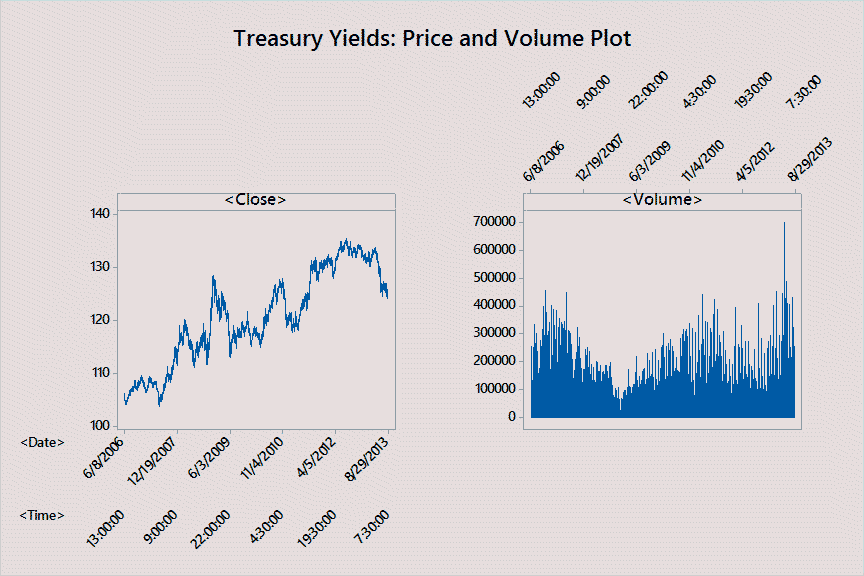
\includegraphics[width=\textwidth]{chapters/chapter_stat_ts/figures/treasury.png}
        \caption{Treasury Yields: Price and Volume Plot \label{fig:treasuryyields}}
        \end{figure}
        
        \begin{figure}[!ht]
        \centering
        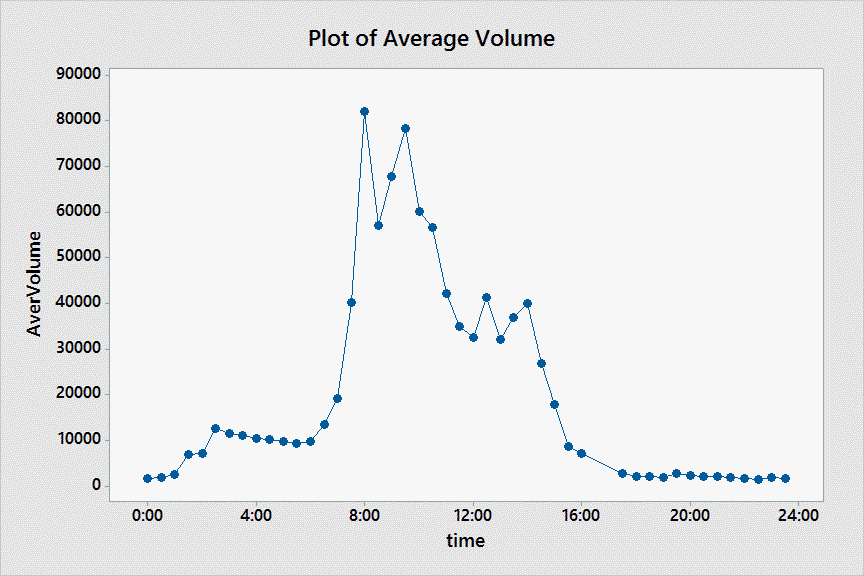
\includegraphics[width=\textwidth]{chapters/chapter_stat_ts/figures/avgvol.png}
        \caption{Plot of average volume. \label{fig:averagevolume}}
        \end{figure}

The plot of price and volume data is given in Figure~\ref{fig:treasuryyields}. The price data generally shows an upward trend, but it is difficult to see the pattern in volume, especially during the course of the day. A simple average volume plot clearly indicates most of the trading occurs between 8~a.m. and 4~p.m. (Figure~\ref{fig:averagevolume}). The autocorrelation function of the log volume ($v_{tm}$) clearly demonstrates the intra-day variations in the data. There is a great deal of interest among practitioners to model the volume accurately as volume is commonly used in a trading strategy, VWAP assumes that volume is known apriori. Two other benefits cited in Satish, Saxena and Palmer (2014)~\cite{satish} are if a trader receives a large order ten minutes before the close with an instruction to complete the order, having a reliable estimate of expected volume can help evaluate the feasibility of that order execution. The other benefit that is mentioned is how improved volume forecast can aid alpha capture. Brownlees, Cipollini and Gallo (2011)~\cite{brownless} propose a dynamic model,
	\begin{equation} \label{eqn:dynamic}
	V_{tm}= \eta_t \cdot \phi_m \cdot \mu_{t.m} \cdot \epsilon_{t.m},
	\end{equation}
where $\eta_t$ is a daily component, $\phi_m$ is the periodic component and $\mu_{t.m}$, an intra-daily dynamic, non-periodic component. The periodic component $\phi_m$ modeled as a Fourier (sine/cosine) function; the daily component is modeled as a function of past values of daily volumes and the same is true with $\mu_{t.m}$; they are modeled as a function of $\mu_{t.m-1}$ and $V_{t.m-1}$. From the structure of the model \eqref{eqn:dynamic}, it is obvious that the multiplication components can be modeled additively through log transformations.


We suggest a model somewhat similar to \eqref{eqn:dynamic} but more directly related to models discussed in Chapter~\ref{ch:ch_uvts}. Before we state the results recall the main findings from past empirical studies:
	\begin{itemize}
	\item Volatility, measured by returns squared is positively correlated with volume.
	\item Large price movements are followed by high volume.
	\item Conditioning on lagged volume attenuates the leverage effect.
	\item After conditioning on lagged volume, there is positive risk-return relationship
	\end{itemize}
Our approach to modeling is stated as follows:
	\begin{itemize}
	\item Model the volume at different frequency levels.
	\item Use the low frequency data for developing macro strategies.
	\item Use the high frequency data for making micro decisions.
	\end{itemize}

        \begin{figure}[!ht]
        \centering
        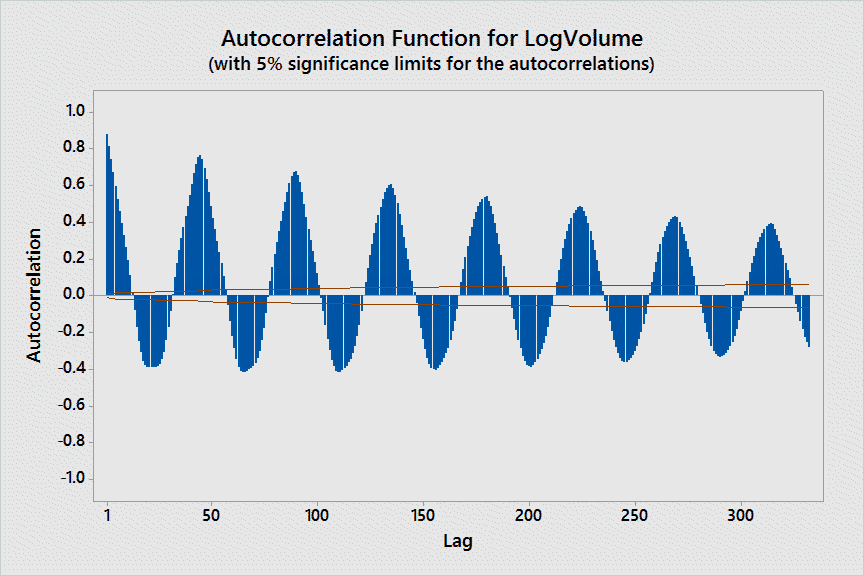
\includegraphics[width=\textwidth]{chapters/chapter_stat_ts/figures/logvol.png}
        \caption{Autocorrelation function for log volume. \label{fig:logvolumeauto}}
        \end{figure}
        
        \begin{figure}[!ht]
        \centering
        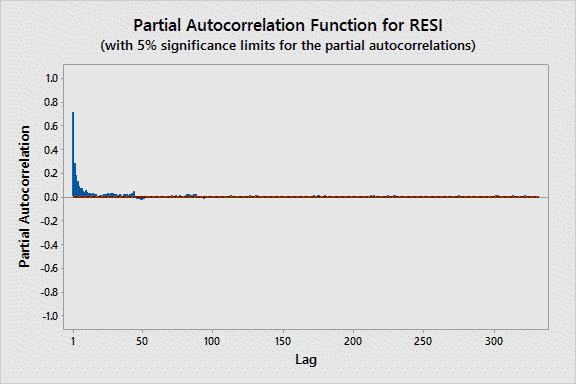
\includegraphics[width=\textwidth]{chapters/chapter_stat_ts/figures/resi.png}
        \caption{Partial autocorrelation function for RESI (with 5\% significance limits for the partial autocorrelations) \label{fig:partresi}}
        \end{figure}
        
        \begin{figure}[!ht]
        \centering
        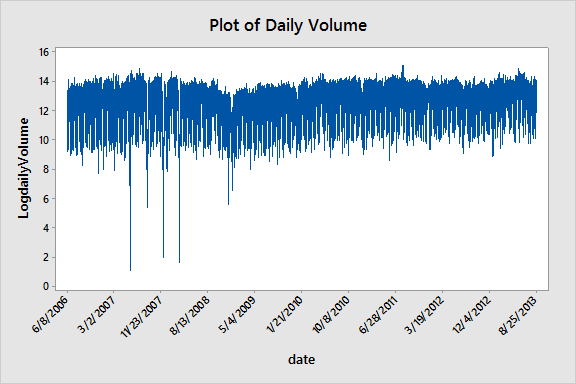
\includegraphics[width=\textwidth]{chapters/chapter_stat_ts/figures/dailyvol.png}
        \caption{Plot of daily volume. \label{fig:dailyvol}}
        \end{figure}


Given the strong intra-day periodicity that is evident from Figure~\ref{fig:logvolumeauto}, we can simply create indicator variables for the 30-min periods and regress the volume on the indicators to capture the time of the day variation. This explains almost sixty-five percent of the variation in log volume. The residuals capture non-periodic patterns and the partial autocorrelation function is given in Figure~\ref{fig:partresi}. This suggests that the residuals can be modeled as higher order autoregressive process. As these components are additive, the forecasts from indicator regression and this autoregression of residuals can be summed up, to arrive at a reasonable volume forecast. The plot of logged daily volume is given in Figure~\ref{fig:dailyvol} and it is clearly stationary. The partial autocorrelation function in Figure~\ref{fig:logdailyvolume} has somewhat a simpler structure for the daily aggregated data. 


How do we use these results optimally?
	\begin{itemize}
	\item Forecast next day volume using the macro model.
	\item Forecast the 30-min volume using the micro model.
	\item If the actual volume is not in line with the forecast, search if any new information has arrived!
	\end{itemize}
	
	
These methods obviously require the use of time series programs and as an alternative approximation, we suggest using exponential smoothing approach. The details are as follows:
	\begin{itemize}
	\item Volume Forecast 1 (Direct): Use daily data to forecast $\hat{v}_{t+1}$, next day's volume; use exponential smoothing constant in the range of 0.25--0.35.
	\item Volume Forecast 2 (Aggregated): We will use a two-step procedure here:
		\begin{enumerate}[(a)]
		\item Compute the average volume $\overline{v}$ over certain number of days for each `$m$'. Usually industry uses `22' days.
		\item Compute the residuals: $e_{t\cdot m} = v_{t . m} - \overline{v}$; use exponential smoothing on $e_{t\cdot m}$ with a smoothing constant in the range of 0.25--0.35; estimate $\hat{e}_{t+1 . m}$;
		\item Forecast for next period `$m$': $\hat{v}_{t+1. m}=\overline{v}+\hat{e}_{t+1 . m}$
		\item Aggregate $\hat{v}_{t+1\cdot m}$ over $m$ to get $\hat{v}_{t+1}$. 
		\end{enumerate}
	Now we have two forecasts of daily volume $\hat{v}_{t+1}$ and $\hat{v}_{t+1}$.
	\end{itemize}
We want to relate the volume to volatility using the measure in \eqref{eqn:hatsigmasq}. Figure~\ref{fig:30min}, based on the plot of Figure~\ref{fig:dailyvol} indicates that there are clustering effects. From the partial autocorrelation function given in Figure~\ref{fig:funvol}, there is some memory in the variance and can be modeled via GARCH. Here our goal is to show how volume and volatility are likely to be related. The simple cross-correlation function, Figure~\ref{fig:ccresi}, shows how they are closely related; here the intra-day periodicity in the residuals in volume and volatility is shown. Again in the spirit of intuitive approach to model the volatility, we suggest obtaining volatility forecasts as:
	\[
	\begin{cases}
	\hat{\sigma}_{t+1}^2 = \text{ weighted average of } \sigma_t^2, \sigma_{t-1}^2, \ldots, \sigma_{t-22}^2 & \\
	\hat{\sigma}^2_{t+1 \cdot m}= \text{ weighted average of } \sigma_{t\cdot m}^2, \sigma_{t-1 \cdot m}^2, \ldots, \sigma_{t-22\cdot m}^2 & 
	\end{cases}
	\]
The following algorithm that combines the price, volume and volatility is suggested; we assume that price-based rules given in Section~\ref{s:trading_rules_tad} are followed.
	\begin{itemize}
	\item Enter if \\
	(a) price-based rules favours and if \\
	(b) $\sigma_{t+1\cdot m}^2< \hat{\sigma}_{t+1\cdot m}^2$, (realized volatility $<$ predicted volatility) and if \\
	(c) $\sum_{i=1}^m v_{t+1} < \sum_{i=1}^m \hat{v}_{t+1}$, cumulative actual volume $<$ cumulative predicted volume. 
	\item Exit if either (a) or (b) or (c) is not true. 
	\end{itemize}
	
        \begin{figure}[!ht]
        \centering
        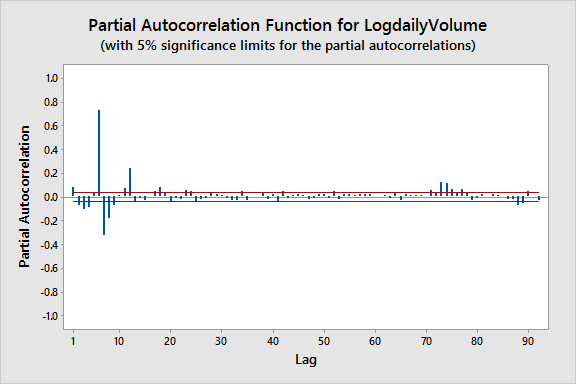
\includegraphics[width=\textwidth]{chapters/chapter_stat_ts/figures/logdaily.png}
        \caption{Partial autocorrelation function for log daily volume (with 5\% significance limits for the partial autocorrelation). \label{fig:logdailyvolume}}
        \end{figure}
        
        \begin{figure}[!ht]
        \centering
        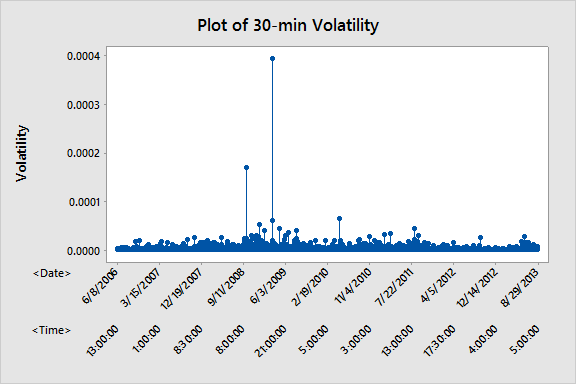
\includegraphics[width=\textwidth]{chapters/chapter_stat_ts/figures/30min.png}
        \caption{Plot of 30-min volatility. \label{fig:30min}}
        \end{figure}
        
        \begin{figure}[!ht]
        \centering
        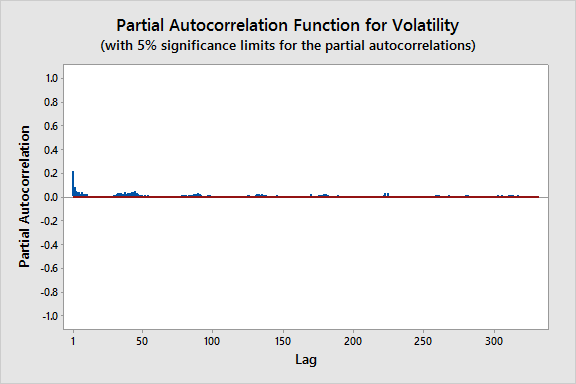
\includegraphics[width=\textwidth]{chapters/chapter_stat_ts/figures/funvol.png}
        \caption{Partial autocorrelation function for volatility (with 5\% significance limits for the partial autocorrelations). \label{fig:funvol}}
        \end{figure}
        
        \begin{figure}[!ht]
        \centering
        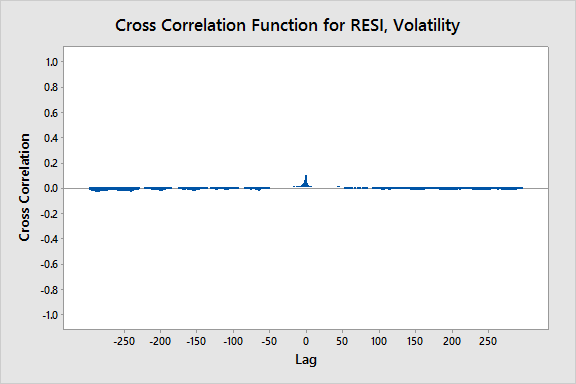
\includegraphics[width=\textwidth]{chapters/chapter_stat_ts/figures/resivol.png}
        \caption{Cross correlation function for RESI, volatility. \label{fig:ccresi}}
        \end{figure}



% Trading in Multiple Markets
\section{Trading in Multiple Markets}

There has been a great deal of interest in studying the performance of cross-listed stocks in several markets, that operate in overlapping or in non-overlapping hours during a day. Both in NYSE and in NASDAQ the listing of non-US firms has increased over time. The general motivation behind cross-listings is to manage the capital raising cost. Some unique features of trading these stocks include the trading hours and restrictions on moving capital from one market to other, and time needed to set up money transfer arrangements that are usually handled through an issuing investment bank. But our focus here is to study the imperfect pricing that may arise from cross-listed markets and see how trading opportunities in these markets can be exploited. More broadly it is of interest to study the information flow from one market to other.


The foreign companies list shares for trading in exchanges in US in the form of ADR (American Deposit Receipts) that ensures the convertibility of home-market shares in US shares and back again. There is generally no conversion fee and there may be restrictions on cross-country ownership. Gagnon and Karolyi (2010)~\cite{gagkar} investigate arbitrage opportunities in these markets by comparing intraday prices and quotes and observe that price parity deviation is quite small (4.9 basis points) but can reach large extremes when the markets are volatile. 


To model the price (co)movements in a calendar day when exchanges operate, the hours can be stated in terms of GMT:
\begin{figure}[!ht]
   \centering
	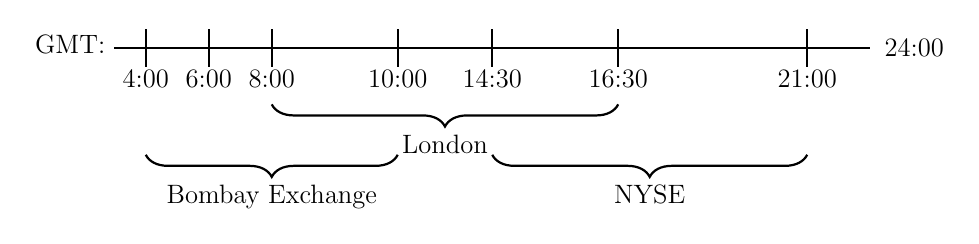
\begin{tikzpicture}[thick,scale=0.8, every node/.style={transform shape}]
	\draw[thick] (-10,0) -- (2,0);
	
	\draw[thick] (-9.5,-0.3) -- (-9.5,0.3);
	\draw[thick] (-8.5,-0.3) -- (-8.5,0.3);
	\draw[thick] (-7.5,-0.3) -- (-7.5,0.3);
	\draw[thick] (-5.5,-0.3) -- (-5.5,0.3);
	\draw[thick] (-4,-0.3) -- (-4,0.3);
	\draw[thick] (-2,-0.3) -- (-2,0.3);
	\draw[thick] (1,-0.3) -- (1,0.3);
	
	\node at (-9.5,-0.5) {\large{4:00}};
	\node at (-8.5,-0.5) {\large{6:00}};
	\node at (-7.5,-0.5) {\large{8:00}};
	\node at (-5.5,-0.5) {\large{10:00}};
	\node at (-4,-0.5) {\large{14:30}};
	\node at (-2,-0.5) {\large{16:30}};
	\node at (1,-0.5) {\large{21:00}};
	
	\node at (-10.7,0.05) {\large{GMT:}};
	\node at (2.7,0) {\large{24:00}};
	
	\draw [decorate,decoration={brace,amplitude=8pt,mirror},xshift=0pt,yshift=0pt]
(-7.5,-0.9) -- (-2,-0.9) node [below=20pt,black,midway,xshift=0cm,yshift=0.35cm] {\large{London}};
	\draw [decorate,decoration={brace,amplitude=8pt,mirror},xshift=0pt,yshift=0pt]
(-4,-1.7) -- (1,-1.7) node [below=20pt,black,midway,xshift=0cm,yshift=0.35cm] {\large{NYSE}};
	\draw [decorate,decoration={brace,amplitude=8pt,mirror},xshift=0pt,yshift=0pt]
(-9.5,-1.7) -- (-5.5,-1.7) node [below=20pt,black,midway,xshift=0cm,yshift=0.35cm] {\large{Bombay Exchange}};
	
	\end{tikzpicture} 
   \caption{Opening hours of some stock exchanges. \label{fig:openingmarket}}
\end{figure}
Denoting the ADR returns as $r_{At} = \ln(P_{A,t}) - \ln(P_{A,t-1})$ and the home market returns as $r_{Ht}= \ln(P_{H,t}) - \ln(P_{H,t-1})$, where $P$'s denote the closing prices, the returns are modeled as: 
	\begin{equation} \label{eqn:closeprice}
	r_{A-H.t}= \alpha + \sum_{i= -1}^1 \beta_i^{\text{US}} r_{M,t+i}^\text{US} + \sum_{i= -1}^1 \beta_i^\text{H} r_{M,t+i}^\text{US} + \sum_{i= -1}^1 \beta_i^{Fx} r_{fx.t+i} + a_t.
	\end{equation}
How $r_{A-H.t}= r_{A.t} - r_{H.t}$, $r_M$'s are market indices and $r_{fx}$ is the currency return. Using the standard deviation of the residuals, `$a_t$', as an idiosyncratic risk proxy in the model \eqref{eqn:closeprice} results from Gagnon and Karolyi (2010)~\cite{gagkar} indicate `the presence of important sources of excess comovement of arbitrage returns with market index and currency returns.' \twomedskip



\noindent\textbf{Dynamic Linkages Across Vector Time Series:} As observed, some markets operate at times that may or may not overlap with others. On any given calendar day, for example, Asian markets open and close before the US markets. Efficient market theory would suggest that all available information about a stock would be impounded in the stock price and there should be no systematic lagged inter-market adjustments that can be exploited. But empirical studies reveal that there could be significant correlations across markets, during the same calendar day and possibly in lagged relationships as well. This phenomenon is also known as \emph{data synchronization problem}. Some studies focus on the overlapping durations between two markets if they exist (for example between London and NYSE), but the information flow during overlapping and non-overlapping periods may not be processed similarly. 


To motivate, consider two markets that do not overlap and let us denote the closing log prices as, $p_t = (p_{1t}, p_{2t})'$; if the markets are efficient and operate independently, each component of $p_t$ will follow a random walk model; but if there is any dependency, it is usually captured by the cointegrating relationship among the components as in pairs trading set-up. We will assume that $p_{2t}$ occurs after $p_{1t}$ in a calendar day, `$t$'. Koch and Koch (1991)~\cite{kochsq} discuss a dynamic simultaneous equations model that takes into account both the contemporaneous and the lead-lag relationships. In its simplest form, the model can be stated as,
	\begin{flalign} \label{eqn:matrixeq}
	&&\begin{pmatrix} 1 & 0 \\ -\phi_{21} & 1 \end{pmatrix}  \begin{pmatrix} p_{1t} \\ p_{2t} \end{pmatrix} &= \begin{pmatrix} \phi_{11} & \phi_{12} \\ 0 & \phi_{22} \end{pmatrix} \begin{pmatrix} p_{1t-1} \\ p_{2t-1} \end{pmatrix} + \begin{pmatrix} a_{1t} \\ a_{2t} \end{pmatrix} && \notag \\
	\text{or} && \phantom{x} & \phantom{x} && \\
	&& \Phi_{01} p_t &= \Phi_{11} p_{t-1} + a_t&& \notag
	\end{flalign}


With four elements in $\Phi_1^*$, one in $\Phi_{01}$ and three in $\Phi_{11}$ are exactly identified. Note  if we denote $\Phi^{-1}_{01} = (\phi_{01},\phi_{02})$ and $\Phi_{11} = \begin{pmatrix} \phi_{11}' \\ \phi'_{21} \end{pmatrix}$ when $\phi$'s are $2 \times 1$ column vectors, $\Phi_1^*=\phi_{01}\phi_{11}' + \phi_{02} \phi_{21}'$  is the sum of two rank one matrices. One could use rank factorization to identify the element $\phi_{21}$ and the elements in $\Phi_{11}$ as well. 


Extending the model in \eqref{eqn:matrixeq} to say `$m$' markets, we can observe that the same-day cross-market linkages are reflected in the matrix, $\Phi_{01}$ and lagged linkages are reflected in the elements of the matrix, $\Phi_{11}$. Let $Y_t = (y_{1t} ,\ldots, y_{mt})'$ denote the time series data at `$t$' and the VAR(1) model takes the form,
	\begin{equation} \label{eqn:formtake}
	\Phi_{01} Y_t= \Phi_{11} Y_{t-1} + a_t,
	\end{equation}
where $a_t$ is a white noise sequence; we will assume that
	\[
	\Phi_{01}= \begin{pmatrix} 
	1 & 0 & \cdots & 0 & 0 \\
	-\phi_{21} &  1 & \cdots & 0 & 0 \\
	\vdots & \vdots &  \ddots & \vdots & \vdots \\
	\vdots & \vdots & & 1  & 0 \\
	-\phi_{m1} & -\phi_{m2} & \cdots & -\phi_{m(m-1)} &  1 
	\end{pmatrix} \enskip \text{ and } \enskip
	\Phi_{11}= \begin{pmatrix}
	\phi_{11} &  \phi_{12} &  \cdots & \phi_{1m} \\
	0 & \phi_{22} & \cdots & \phi_{2m} \\
	\vdots & \vdots & \ddots & \vdots \\
	0 & 0 & \cdots & \phi_{mm} 
	\end{pmatrix}
	\]
are triangular matrices with $\frac{(m-1)m}{2}+ \frac{(m+1)m}{2}$ elements that add up to $m^2$ elements that result from a regular VAR(1) model, given below and thus the elements of $\Phi_{01}$
and $\Phi_{11}$ are clearly identified. 


Note \eqref{eqn:formtake} can be written as,
	\begin{equation} \label{eqn:rewrittenas}
	Y_t= \Phi_{01}^{-1} \Phi_{11} Y_{t-1} + \Phi_{01}^{-1} a_t = \Phi_1 Y_{t-1} + \epsilon_t,
	\end{equation}
which is the VAR(1) model with no simultaneous dependence in $Y_t$. But observe that $\epsilon= \Phi_{01}^{-1} a_t$ contains information about $\Phi$ and in model \eqref{eqn:formtake} we do assume that  $a_{jt}$ is independent of $(a_{1t},\ldots, a_{(j-1)t})$ for $j = 2,\ldots,m$.


It can be shown that $\Phi_1= \Phi_{01}^{-1} \Phi_{11}$ is the sum of `$m$' rank one matrices. Again, the identification of the elements of $\Phi_{01}$ and $\Phi_{11}$ from $\Phi_1$ is fairly straightforward. The number of elements in $\Phi_{01}$ and the number in $\Phi_{11}$ add up to $m^2$, the number of elements in $\Phi_1$. Also observe that the model \eqref{eqn:formtake} can be still written as VAR(1) model, in $\Phi_{01} Y_t$,
	\begin{equation} \label{eqn:var1phimod}
	\Phi_{01} Y_t = \Phi_{11} \Phi_{01}^{-1} ( \Phi_{01} Y_{t-1}) + a_t
	\end{equation}
for a known $\Phi_{01}$.


As indicated in Chapter~\ref{ch:ch_mvts}, for the stationarity of the VAR(1) model, it is required that the eigenvalues of $\Phi_1$, i.e., $\det(\Phi_1 - \lambda I)= \prod_{j=1}^m (1-\lambda_j)$, where $|\lambda_j| \leq 1$ for all `$j$'. Recall that the properties of the non-stationary series, that is, when some of the eigenvalues, $|\lambda_j|$ are unity. Relate to the canonical correlations between $Y_t$ and $Y_{t-1}$. The canonical correlations are obtained as the eigenvalues of the matrix, $(\Gamma_0^{- \frac{1}{2}} (y)\, \Phi_1 \,\Gamma_0^{\frac{1}{2}}(y)) ( \Gamma_0^{\frac{1}{2}}(y) \,\Phi_1'\,  \Gamma_0^{-\frac{1}{2}}(y))$, when $\Gamma_0(y)$ is the variance-covariance matrix of $Y_t$. Reinsel and Velu (1998)~\cite{velurein} have shown that this is equivalent  to connecting the eigenvalues of $\Phi_1$, $\lambda(\Phi_1)= \lambda( \Gamma_0^{-\frac{1}{2}} (y) \,\Phi_1\, \Gamma_0^{\frac{1}{2}}(y))= \lambda(\Phi_1^*)$ with the singular values of $\Phi_1^*$, $\sigma(\Phi_1^*)$. 


Some research issues are: 


\begin{enumerate}[--]
\item How do we identify the triangular coefficient matrices, both contemporaneous and the lagged, from the general VAR(p) coefficient matrices?
\item What is the effect of ignoring the contemporaneous dependence on the estimation of co-integrating relationships?
\item For select Indian stocks does it make any difference in forecasting the price direction based on information flows by accounting for the data synchronization?
\end{enumerate}
The last aspect is studied here. 


        \begin{figure}[!ht]
        \centering
        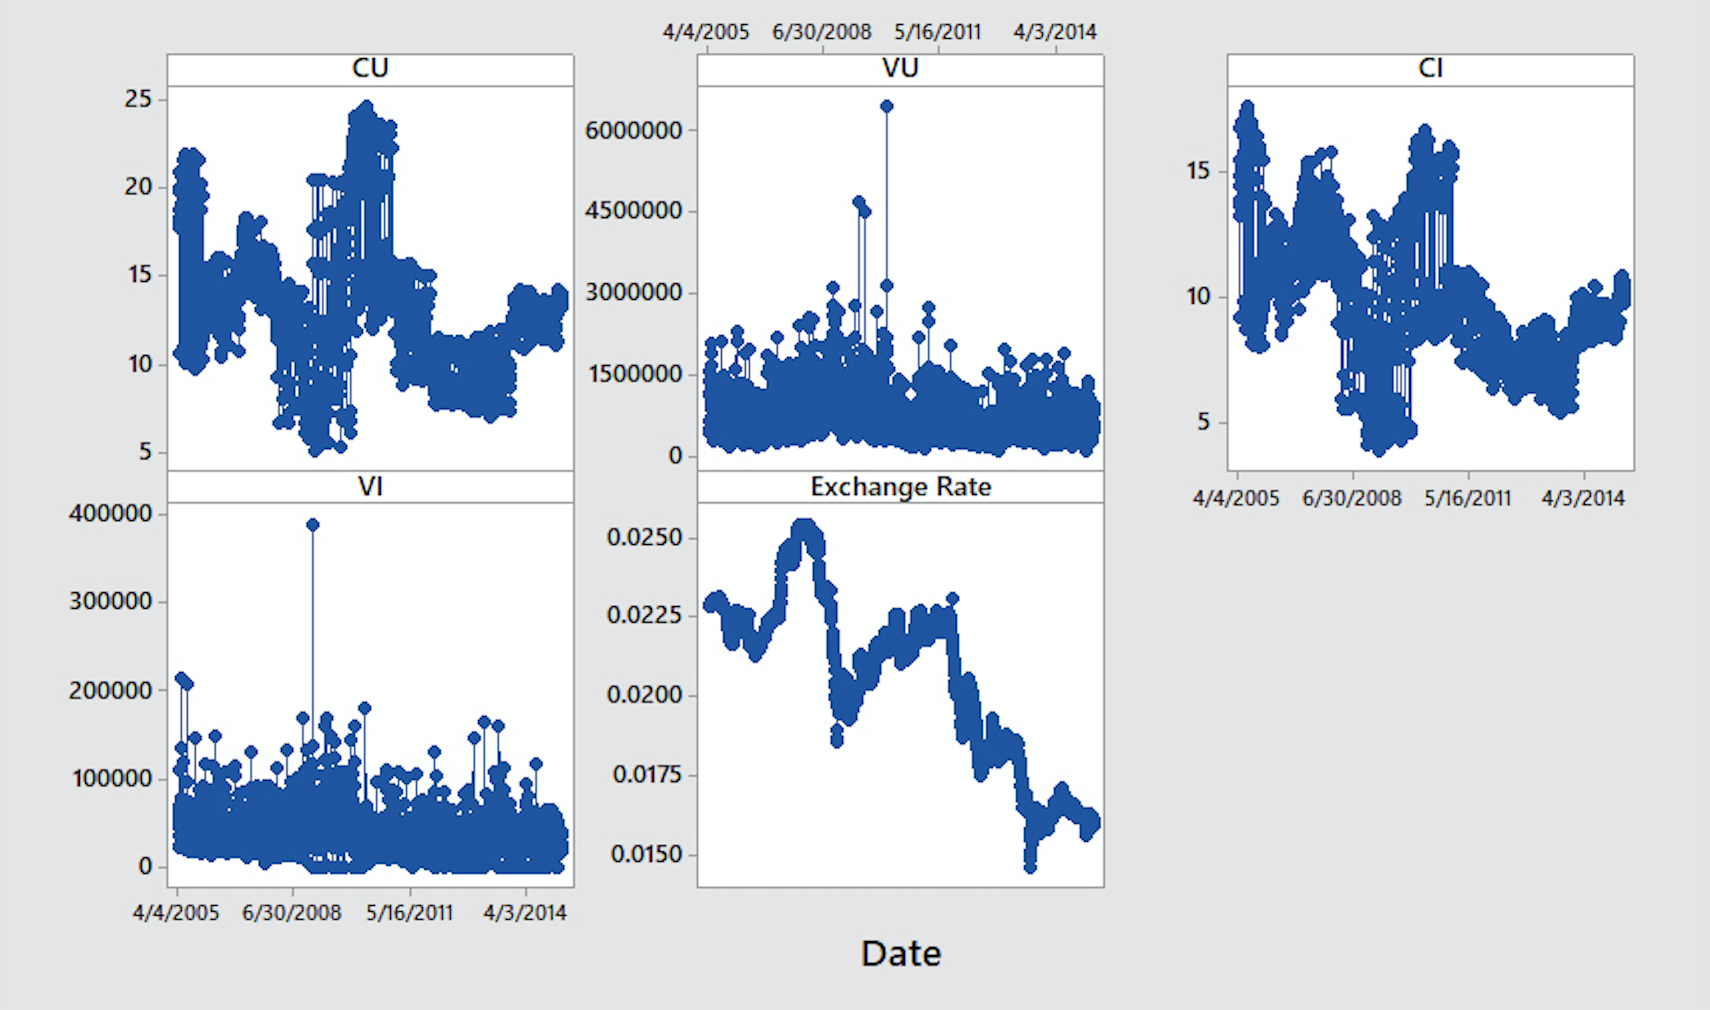
\includegraphics[width=\textwidth]{chapters/chapter_stat_ts/figures/cpver.png}
        \caption{Plot of closing prices, volumes and exchange rates. \label{fig:cpver}}
        \end{figure}


To illustrate we consider the data on WIPRO---an Indian stock that is traded in both US and Bombay markets. The plot of the closing prices in both markets (CU---closing price in US market, VU---volume in US market, etc.) is given in Figure~\ref{fig:cpver}. The exchange rate has been generally in favor of a dollar during this period (2005--2014), but the volatility is higher in the US market. To illustrate the flow of information in one market to another we fit the following models; let $p_{1t}$ be the log closing price in India and $p_{2t}$ be the log closing price in US; Table~\ref{tab:regresul} below summaries the results.
	\begin{table}[!ht] 
	\centering
	\caption{WIPRO regression results \label{tab:regresul}}
	\begin{tabular}{l | rr} 
	& \multicolumn{2}{c}{Response Variable} \\ 
	Predictors & $p_{1t}$ & $p_{2t}$ \\ \hline 
	Constant & $-0.056^*$ & $-0.019^*$ \\
	$p_{1t}$ & ---  & $0.6328^*$ \\
	$p_{1t-1}$ & $0.91^*$ & --- \\
	$p_{2t-1}$ & $-0.026$ & $0.3626^*$ \\ \hline
	$R^2$ & 0.79 & 0.91 
	\end{tabular}
	\end{table}
These results would indicate that the markets are not fully efficient and there is some information transfer from one market to other. The dependence of the US market price on the closing price of the Indian market is clearly evident. This can be favorably used for better US price forecasts. 



% Other Topics: Trade Size etc.
\section{Other Topics: Trade Size etc.}

\noindent \textbf{Trade Size:} \twomedskip

In the trading strategies described above, once entry-exit decisions are made, the size---the number of units to buy and sell---is usually taken to be the total value of the investment. Many traders tend do staggered entry or exit, so that all funds are not invested or taken out at once. The question there is how to determine the size of the bet on each transaction. We want to explore some practical ideas in this section. 


A criterion that is attributed to Kelly (1956)~\cite{kelly56} that was introduced in the context of gambling determines the fraction of investment capital to bet, `$f$', with the initial investment, $X_0$ and `$n$' trials of investment opportunities is based on the wealth accumulation as
	\begin{equation} \label{eqn:xmx01f}
	X_n= X_0(1+fW)^{pn} (1-fL)^{qn},
	\end{equation}
where `$W$' and `$L$' are the number of successes and failures and `$p$' and `$q$' are the respective probabilities. Thus the growth rate per bet is given as
	\begin{equation} \label{eqn:1nln}
	\dfrac{1}{n} \ln \left(\dfrac{X_n}{X_0}\right)= p \ln(1+fW) + q \ln(1-fL)
	\end{equation}
and when maximized results in the optimal bet size as,
	\begin{equation} \label{eqn:fstarp}
	f^*= p - \dfrac{q}{W/L}.
	\end{equation}
In order to implement this in practice, good estimates of `$p$' and `$q$' are needed; the bet size can be revised based on the (recent) empirical observation of `$W$' and `$L$' in the process of investment. A general version of the problem could be to determine the optimal betting vector, $f^*=(f_1^*, \ldots, f_n^*)$, with some dependency structure on the sequential games, but that appears to be complex. 


The usefulness of statistical arbitrage rules can be extended beyond the entry-exit decisions, but the size of entry-exit decisions must be made with alternatives such as investing in risk-free assets. It is shown in Zhu and Zhou (2009)~\cite{zhuzhou09} that when there is uncertainty about the future returns, fixed allocation rules can be enhanced by technical analysis. The fixed allocation rule follows from the portfolio theory presented in Chapter~\ref{ch:amp}. With a single risky asset, whose behavior is monitored through the technical analysis and a risk free asset, the optimal allocation rule follows from Chapter~\ref{ch:amp} as the Sharpe ratio, $w= (\mu - r_f)/\sigma^2$, where $\mu$ and $\sigma^2$ are estimated from the past data and are expected to remain stable in the near future. Assuming that the investor with the initial wealth, $X_0$, wants to maximize the expected value,
	\begin{equation} \label{eqn:euxn}
	E(U(X_n))= E \left[ \dfrac{X_n^{1-\gamma}}{1 - \gamma}\right],
	\end{equation}
where `$\gamma$' is the risk aversion parameter, with the budget constraint,
	\begin{equation} \label{eqn:dxtxt}
	\dfrac{dX_t}{x_t}= r_f \; dt + w_t (\mu_0 + \mu_1 s_t - r_f) \; dt + w_t \sigma \; dB_t.
	\end{equation}
Here it must be observed that $B_t$ is a Brownian motion, $\mu_0$ and $\sigma$ are the mean and standard deviation of the returns and $S_t$ is the state variable that can provide information on the future stock returns. The fixed allocation rate under the assumption that returns are random is
	\begin{equation} \label{eqn:wgamma}
	w(\gamma)= \dfrac{\mu - r_f}{\gamma \cdot \sigma^2}
	\end{equation}
which is the Sharpe ratio adjusted for the risk-aversion. If the information from the state variable, although uncertain, is considered then the optimal investment size is given as
	\begin{equation} \label{eqn:wgamma2}
	w(\gamma)= \dfrac{\mu - r_f}{\gamma \cdot \sigma^2 - (1-\gamma)(d)},
	\end{equation}
where `$d$' depends `$\mu_1$' in \eqref{eqn:dxtxt} that indicates its influence of state variable on the return process and volatility in the state variable; for details see Zhu and Zhou (2009)~\cite{zhuzhou09}. As this quantity `$d$' can take a range of values, the adjustment factor $(1-\gamma)d$ can take positive or negative values. Note when $\gamma=1$, $w(\gamma)= w$, the standard measure of Sharpe ratio. 


To evaluate the additional value of tracking the price over time to decide on the entry strategy, we follow the simple rule based on the moving average of fixed length. If the current price, $p_t$ is greater than the moving average, enter the market:
	\begin{equation} \label{eqn:etatetapt}
	\eta_t= \eta(p_t,A_t)= \begin{cases}
	1, & \text{ if } p_t > A_t \\
	0, & \text{otherwise}
	\end{cases}
	\end{equation}
Under this set-up the optimal bet-size is shown to be
	\begin{equation} \label{eqn:wstarmurf}
	w^*= \dfrac{\mu - r_f}{\sigma^2} + \dfrac{\mu_1}{\sigma^2} \cdot \dfrac{b_1}{b_2},
	\end{equation}
where $b_2=E(\eta_t)$ and $b_1=E((S_t - \overline{S}) \eta_t)$. Observe `$\mu_1$' is the effect of information-based state variable, $S_t$, on the price formation, `$b_2$' is the average number of entries and `$b_1$' provides the average excess of the state variable. While other quantities in \eqref{eqn:wstarmurf} have been historically well-studied, the key ratio that is new here is over $(\mu_1 \cdot b_1)/b_2$ which can be taken as the total size $(\mu_1 b_1)$ can be distributed over `$b_2$' entries. If $\mu_1= 0$, the moving average rule may not add any flexibility to the fixed size entry. 



% Exercises
\section{Exercises}


%Problem
\prob {\it Technical Rules} Consider the data on exchange rates (in file \texttt{rates.csv}) between the Indian Rupee and the US Dollar, British Pound and Euro; it is daily data from December 4, 2006 to November 5, 2010. In order to compare the performance of a strategy, appropriately normalize the entry point exchange rate: invest equal amounts of capital (counted in INR, which we will call the ``base currency'') in each trade. Total portfolio return on each day should be computed as a weighted sum of returns from each active trade (weighted by the current value of each trade). Evaluate the signals discussed in (a) and (b) below using the Sharpe ratios and PNL with and without including transaction costs of $15$ basis points. Assume a risk free rate of $3\%$. (1 basis point = $10^{-4}$; so each dollar traded costs $0.0015$ in transaction costs)
	\begin{enumerate}[(i)]
	\item{\it Moving average trading rules}: Trading signals are generated from the relative levels of the price series and a moving average of past prices.
		\begin{itemize}
		\item  Rule 1: Let $\overline{p}_t^{(m)}$ as defined in \eqref{eqn:multi}; use the strategy to sell if $p_t>\overline{p}_t^{(m)}$ and to buy if  $p_t<\overline{p}_t^{(m)}$. Evaluate this strategy. What is the optimal `$m$'?
		\item Rule 2 (Bollinger rule): Use the Bollinger rule as outlined in the text; what is the optimal `$m$'?
		\item Rule 3 (Resistance-Support): Buy if $p_t > \max_{\substack{0 \leq i< m}} p_{t-i}$ and sell if $p_t < \min_{\substack{0 \leq i < m}} p_{t-i}$. Evaluate this rule. What is the optimal `$m$'?
		\item Rule 4 (Momentum): Compute a short-term moving average over the last $m$ prices, $\overline{p}_t^{(m)}$ and a long-term average over the last $n$ prices, $\overline{p}_t^{(n)}$ with $m<n$. If $\overline{p}_t^{(m)}$ crosses $\overline{p}_t^{(n)}$ from below, sell and if it crosses $\overline{p}_t^{(n)}$ from above, buy. Evaluate this strategy. What are the optimal values of $m$ and $n$?
		\end{itemize}
	\item{\it RSI Oscillator Rule}: Use $\text{RSI}_t$ as defined in \eqref{eqn:rsi}. \hfill \break
If $\text{RSI}_t<30$, buy and if $\text{RSI}_t>70$, sell. Evaluate this trading strategy. What is the optimal `$m$'?

	\item {\it Pairs Trading: Distance Method}

We want to develop a pairs trading strategy and check if it does any better than  the strategies in Problem 1. At the last trading day of the month, look back 3 months and identify if any pairs are worth trading. Use the distance measures, thresholds, as given in the text.

	\item {\it Pairs Trading: Cointegration Method}

In the cointegration method, we can consider the possibility of trading more than 2 assets. Check using a moving window of 3 months which series are cointegrated. Develop appropriate trading strategies to trade portfolios formed from the cointegrating vectors and compare with the pairs trading strategies from based on other criteria. Concretely define the trading indicators and thresholds for entry and exit. Summarize the performance results.

	\item {\it Pairs Trading: APT method}

Consider the data with the S\&P500 market index returns and assume that the risk free rate is 3\%. Regress each currency's excess return (over the risk free rate) on the excess market return over a moving window of 3 months. Find pairs based on the similarity of the regression coefficients.
	\begin{enumerate}
	\item Compare the pairs that result from the APT method with those obtained in Problem 2.
	\item After finding the pairs, use the same rules as in Problem 2 to decide when to enter and exit specific trades.
	\end{enumerate}
Summarize the performance results.

	\item {\it Summing up}

Provide a summary table of portfolio returns of all methods with the main findings and drawbacks of all the methods that are explored in this assignment. In particular, comment on the performance of single-asset strategies versus multi-asset strategies. Also comment on whether the market factor adds any value. \twomedskip
	\end{enumerate}


%Problem
\prob The file Exchange rates.csv contains exchange rates between US\$ and 25 major currencies; the daily data spans from Jan 3, 2000 to April 10, 2012. Consider the data from Jan 3, 2002 for the following currencies: EUR, GBP, DKK, JPY and CNY. Compute $r_t = \ln{p_t} - \ln{p_{t-1}}$, returns for each series. \twomedskip


\indent\textbf{A. Evaluation of Trading Rule:} Consider the data starting June 11, 2003.
	\begin{enumerate}[(a)]
	\item Compute the average return for each day. We will treat this a `market' return.
	\item Consider the two currencies: EURO and JPY and assume that your investment is restricted to only these two currencies. We will follow the simple algorithm: if 
	\[
	\frac{r_i - \overline{r}}{sd(r_i)}=
	\begin{cases}
	>2, & \text{sell} \\
	< -2, & \text{buy} \\
	\text{otherwise}, & \text{hold}
	\end{cases}
	\]
The average and standard deviation of the returns are based on last 30-day observations. Evaluate this algorithm by comparing it with simple holding.
	\item What is the value of the `market' return? How could this information be used?
\end{enumerate}


\textbf{B. Trading Rule with other factors:} In addition to exchange rates from June 11, 2003, consider the data on commodity prices: Gold, Oil, Copper and a commodity index. Among the following currencies, CAD, BRL, ZAR, AUD, NZD, CAF and RUB, which are most influenced by the commodity prices. Discuss how you would incorporate this into a trading strategy. \twomedskip


%Problem 
\prob This is an exercise to replicate the pairs trading strategy. Obtain the daily data from January 2000 to June 2014 on stock prices, returns, trading volume and shares outstanding on the following companies only: \twomedskip

\indent Oil stocks: HAL, SLB, EQT, OXY, CVX \twomedskip

\indent Tech stocks: AAPL, CSCO, GOOG, INTL, MSFT \twomedskip

\indent Bank stocks: BAC, JPM, WFC, C, STI \twomedskip

\indent Retail stocks: ANF, GES, SKS, SHLD, URBN \twomedskip

Begin forming pairs in January 2000 based on the estimation period, January 2000 to December 2000. The last estimation period is January 2014 to December 2014. Eligible pairs corresponding to the last estimation remain eligible till December 2014. Pairs that opened in December 2013 and did not converge with the stipulated maximum of six months would have been closed in June 2014.


As you recall, the pairs trading strategy works as follows:
	\begin{enumerate}[--]
	\item Within each sector, match pairs based on normalized price differences over the past year.
	\item When a tracked pair diverges by more than two standard deviations of their normalized price difference, buy the ``cheap'' stock and sell the ``expensive'' one after a one-day wait period (to mitigate the effects of any market irregularities).
	\item If prices for a traded pair re-converge, exit the paired positions.
	\item If prices for a traded pair do not re-converge within six months, close the positions. An alternative strategy closes all traded pairs in ten trading days.
	\end{enumerate}

\noindent Questions of interest:
	\begin{enumerate}[(a)]
	\item Quantify the profitability of the pairs trading strategy and on average, how long it takes for pairs to re-converge?
	\item Can you provide some insight into why the strategy works based on trading volume, shares outstanding and the market trend?


Another Question of interest
	\item Is there a pair across sectors that can outperform the pairs formed within each sector? \twomedskip
	\end{enumerate}


%Problem
\prob  This is another exercise on `pairs trading' using CRSP data. Obtain the daily data from January 1992 to June 2010 on stock prices, returns, trading volume and shares outstanding on the following companies only:

\indent DELL, HP, ADBE, MSFT, AAPL\hfill \break
\indent JPM, WFC, BAC, C, BRK.A\hfill \break
\indent JNJ, WMT, COST, KO, PEP\hfill \break
\indent GM, TM, F\hfill \break
\indent XOM, COP 

``Begin forming pairs in January 1993 based on the estimation period, January 1992 to December 1992. The last estimation period is January 2009 to December 2009. Eligible pairs corresponding to the last estimation remain eligible till December 2009. Pairs that opened in December 2009 and did not converge with the stipulated maximum of six months would have been closed in June 2010.'' \twomedskip

\noindent Questions of interest:
	\begin{enumerate}[(a)]
	\item Quantify the profitability of the pairs trading strategy and on average, how long it takes for two pairs to reconverge?
	\item Can you provide some insights into why the strategy works based on trading volume, shares outstanding and the market trend? \twomedskip
	\end{enumerate}


%Problem
\prob One of the most intriguing asset pricing anomalies in finance is so-called  ``price momentum effect'' that was covered in this chapter. This exercise using CRSP data is meant to guide you through creating a momentum strategy. The goal is to replicate the price momentum strategy described in Jegadeesh and Titman (2001)~\cite{JeTi} using more recent data extending to December 2014. [This problem is based on the notes from Ravi Jagannathan.] \twomedskip

\textbf{A. Source of Data}
The monthly stock returns from January 1965 to December 2014 can be obtained from the web. You should construct the decile ranking by yourself. For future reference, the decile ranking file is available from Ken French's web site. The NYSE market capitalization decile contains all common shares regardless of the end of the month price.\footnote{The Fama-French factors can be downloaded from Ken French's website. Note that you should only use the data from \textquotedblleft U.S. Research Returns Data\textquotedblright\ section.}You should use each stock's permanent identification code (PERMNO) as a unique identifier for that stock.

Note that not all stocks have valid monthly returns for various reasons. One reason is that the stock gets delisted somewhere during the month. For the construction of your momentum portfolios, you can simply ignore the delisting returns in your portfolio construction and return accumulations for the sake of simplicity. More specifically, for this exercise, if the end of the month return of any stock is missing, you may simply assume the return is zero in your compounding. You should keep track of such cases (identify the reason for delisting/missing observation) and prepare a table summarizing how many such cases occurred. \twomedskip

\textbf{B. Stocks Selection Criterion}
Consider all the common stocks traded on AMEX, NYSE and NASDAQ but
subject to the following filtering rules:
	\begin{itemize}
	\item Exclude all stocks priced lower than $\$5$ at the end of month ($t$).
	\item Exclude all stocks belonging to the smallest NYSE market decile at the end of month ($t$). You should first find the cutoff for the NYSE smallest market decile, then delete all the stocks (including stocks on AMEX, NYSE, and NASDAQ) with a market cap that's below the cutoff.
	\item Another thing to take in consideration is that when you form your portfolios, you should only apply the filters to the stocks when you form the portfolio (i.e. at the end of month $t$). The future returns (stock returns at month $t+2$ to $t+7$) should not be filtered. Otherwise it creates a look-ahead bias. For example, for portfolio returns at month $t+2$ to $t+7$, you drop stocks with a price $<$5 at any month between $t+2$ to $t+7$. First, when forming the portfolio at time t, you use information you don't have at month t. Second, you eliminate stocks with likely poor performance (low price) in the future. The portfolio returns (especially the loser portfolio returns) are likely to be biased upward from this action. \twomedskip
\end{itemize}


Again, you should keep track of such cases and prepare a table summarizing how many such cases occurred. \twomedskip

\textbf{C. Portfolio Formation}
At the end of each month ($t$), sort the stocks into $10$ decile portfolios based on the six month cumulative returns between month ($t-5$) to ($t$). The first decile contains the stocks with the lowest past six-month returns, and the tenth decile contains the stocks with the highest past six-month returns.
	\begin{itemize}
	\item Start by accumulating the return of each decile portfolio between ($t+2$) to ($t+7$), i.e. skipping the first month following the portfolio
formation.
	\item At the beginning of each month, construct overlapping decile portfolios as equally weighted averages of the past six month months' decile portfolios. That is, at each month $\tau $, the $i$th overlapping decile portfolio consists of an equal weighted average of the\ $i$th decile portfolios of the previous six month ($\tau -5$) to ($\tau $).\footnote{These 10 overlapping decile portfolios are the testing assets in our asset
pricing test exercises.}
	\item For each month and of the 10 overlapping decile portfolios, record the portfolio returns between January 1995 and December 2014. \twomedskip
	\end{itemize}

\textbf{D. Questions of Interests}
After constructing the relevant portfolios, answer the following questions. When you answer these questions, note any additional assumptions/choices you made. \twomedskip


\textbf{Momentum strategy profits.}
	\begin{enumerate}[a.)]
	\item Report the monthly average returns of your overlapping decile portfolio, as well as the winner ($P1$, highest past six month return portfolios) minus losers ($P10$, lowest past six month return portfolios).
	\item Report the monthly average returns of your overlapping decile portfolio for January and non-January months respectively, as well as the winner ($P1$, highest past six month return portfolios) minus losers ($P10$, lowest past six month return portfolios).
	\item Using CAPM and Fama-French version of multifactor asset pricing model to test the spreads between winner and loser portfolio ($P10$ - $P1$). \ The Fama-French factors can be obtained from Kent French's web site.
	\item Tabulate these results in a table similar to table $I$ in Jegadeesh and Titman (2001)~\cite{JeTi}.
	\item Compared your results to the results in Jegadeesh and Titman (2001)~\cite{JeTi} \emph{and comment on your findings.} \twomedskip
	\end{enumerate}

\textbf{Momentum strategy and market capitalization:}
	\begin{enumerate}
	\item[f.)] Repeat the above exercise but split the sample into small-cap and big-cap portfolio, where the small-cap portfolio contains the stocks in the lower five NYSE market capitalization deciles.
	\item[g.)] Tabulate these results in a table similar to table $I$ in Jegadeesh
and Titman (2001)~\cite{JeTi}.
	\item[h.)] Compare the simple momentum strategy's profits, and momentum strategy cut by the market capitalization profits to value-growth strategy's return. The value-growth strategy return can be proxied by the HML factor obtained from Ken French's website.
	\item[i.)] \emph{Comment on your findings}. In particular, briefly suggest at least three reasons why momentum profits may be related to market capitalization, and how would you go ahead and test it further. \twomedskip
	\end{enumerate}


%Problem
\prob This is another exercise using data for sixteen stocks to replicate the price momentum strategy albeit in a small scale.The daily returns from January 11, 2000 to November 20, 2005 for sixteen stocks are in the file \texttt{d\_logret\_16stocks};
to this add two more columns: SP500 returns and risk free rate.
    \textbf{Portfolio Formation:} \hfill \break
    On the last day of each month, sort the stocks into four quartile portfolios based on the past six month
cumulative returns. The first quartile contains the stocks with the lowest past six-month returns, and the
fourth quartile contains the stocks with the highest past six-month returns.
        \begin{enumerate}[(a)]
        \item Start by accumulating the return of each quartile portfolio for next six months
        \item For each month and of the four quartile portfolios, record the average portfolio returns between January 2002 and November 2005.
        \end{enumerate}
    \textbf{Questions of Interests} \hfill \break
    Same as in Exercise~5. \twomedskip


%Problem
\prob Consider the 30~min price bar data for Treasury Yields from June 8, 2006 to August 29, 2013. Daily data for Treasury Yields is just a snapshot at 4~p.m. and the total volume for the day is the sum of 30~min volumes since the previous day. This is the same data used in Section~\ref{sec:illus_ex} in the text.
   \begin{enumerate}[(a)]
   \item Develop ARMA time series models for both daily and the 30~min volumes. We can use daily data
for developing macro strategies and 30~min data for micro strategies.
\item Compare the exponential smoothing approach suggested in the text with ARMA modeled in (a).
   \item Compute volatility measure, $\sigma_t^2 = 0.5[\ln{\frac{H_t}{L_t}}]^2 - 0.386[\ln{\frac{C_t}{O_t}}]^2$ for both daily and 30~min levels and compare them
   \item Compute volatility forecasts, $\hat{\sigma}_{t+1}^2$ = weighted average of $\sigma_{t}^2, \sigma_{t-1}^2,...,\sigma_{t-22}^2$, for daily data and $\hat{\sigma}_{t+1\cdot m}^2$ = weighted average of $\sigma_{t\cdot m}^2,...,\sigma_{t-22\cdot m}^2$ for $m^{th}$ 30-min interval. [ In (a), you should notice strong seasonality in the 30-min data]
   \item Develop trading strategies that incorporate
      \begin{enumerate}
      \item price information only
      \item price and volume information and
      \item price, volume and volatility information
      \end{enumerate}
         \item Demonstrate that volume and volatility add value to the enter/exit strategies. \twomedskip
   \end{enumerate}